% =====================================================================
% LATTICE9 — Distributed Adversarial Graph-Computation Engine
% Probabilistic Topology Reasoning Framework
% Technical Whitepaper v9.0.0-PRO-CLAW
% =====================================================================
\documentclass[11pt,a4paper]{article}

% ── Packages ─────────────────────────────────────────────────────────
\usepackage{graphicx}
\usepackage{xcolor}
\usepackage{geometry}
\usepackage{amsmath,amssymb,amsthm}
\usepackage{mathtools}
\usepackage{bm}
\usepackage{booktabs}
\usepackage{enumitem}
\usepackage{tabularx}
\usepackage{adjustbox}
\usepackage{longtable}
\usepackage{fancyhdr}
\usepackage{titlesec}
\usepackage{tcolorbox}
\tcbuselibrary{skins,breakable}
\usepackage{listings}
\usepackage{microtype}
\usepackage{float}
\usepackage{caption}
\usepackage{subcaption}
\usepackage{multicol}
\usepackage{alphalph}

% ── Colors (before hyperref) ────────────────────────────────────────
\definecolor{indigo}{HTML}{2C3E6B}
\definecolor{indigolight}{HTML}{5A6A9A}
\definecolor{indigopale}{HTML}{E8EBF2}
\definecolor{theoremgray}{HTML}{F5F5F8}
\definecolor{darktext}{HTML}{1A1A2E}
\definecolor{midgray}{HTML}{6B7280}
\definecolor{lightgray}{HTML}{E5E7EB}
\definecolor{codebg}{HTML}{F8F9FC}

% ── Geometry ─────────────────────────────────────────────────────────
\geometry{a4paper, top=2.5cm, bottom=2.5cm, left=2.5cm, right=2.5cm}

% ── Fonts (XeLaTeX/Tectonic) ────────────────────────────────────────
\usepackage{fontspec}
\setmainfont{Liberation Serif}[
    BoldFont = Liberation Serif Bold,
    ItalicFont = Liberation Serif Italic,
    BoldItalicFont = Liberation Serif Bold Italic,
]
\setsansfont{Carlito}[
    BoldFont = Carlito Bold,
    ItalicFont = Carlito Italic,
]
\setmonofont{Sarasa Mono SC}[
    Scale = 0.88,
]

% ── Hyperref (LAST content package) ──────────────────────────────────
\usepackage[
    colorlinks=true,
    linkcolor=indigo,
    citecolor=midgray,
    urlcolor=indigo,
    bookmarks=true,
    bookmarksnumbered=true,
    unicode=true
]{hyperref}

% ── Header / Footer ─────────────────────────────────────────────────
\pagestyle{fancy}
\fancyhf{}
\setlength{\headheight}{14pt}
\fancyhead[L]{\footnotesize\textsf{\textcolor{midgray}{LATTICE9}}}
\fancyhead[C]{\footnotesize\textsf{\textcolor{midgray}{TECHNICAL WHITEPAPER}}}
\fancyhead[R]{\footnotesize\textsf{\textcolor{midgray}{v9.0.0-PRO-CLAW}}}
\fancyfoot[L]{\footnotesize\textsf{\textcolor{midgray}{Open Systems Architecture Research}}}
\fancyfoot[C]{\footnotesize\textsf{\textcolor{midgray}{\thepage}}}
\fancyfoot[R]{\footnotesize\textsf{\textcolor{midgray}{Reference Architecture}}}
\renewcommand{\headrulewidth}{0.3pt}
\renewcommand{\headrule}{\hbox to\headwidth{\color{indigolight}\leaders\hrule height \headrulewidth\hfill}}
\renewcommand{\footrulewidth}{0.3pt}
\renewcommand{\footrule}{\hbox to\headwidth{\color{indigolight}\leaders\hrule height \footrulewidth\hfill}}

% ── Section Styling ──────────────────────────────────────────────────
\titleformat{\section}
    {\normalfont\Large\sffamily\bfseries\color{indigo}}
    {\thesection}{1em}{}[\vspace{-0.5em}\textcolor{indigolight}{\rule{\textwidth}{0.4pt}}]

\titleformat{\subsection}
    {\normalfont\large\sffamily\bfseries\color{darktext}}
    {\thesubsection}{1em}{}

\titleformat{\subsubsection}
    {\normalfont\normalsize\sffamily\bfseries\color{midgray}}
    {\thesubsubsection}{1em}{}

% ── Theorem Environments ─────────────────────────────────────────────
\theoremstyle{definition}
\newtheorem{definition}{Definition}[section]
\newtheorem{theorem}{Theorem}[section]
\newtheorem{lemma}[theorem]{Lemma}
\newtheorem{proposition}[theorem]{Proposition}
\newtheorem{corollary}[theorem]{Corollary}

% ── tcolorbox Styles ─────────────────────────────────────────────────
\newtcolorbox{theorembox}[1][]{
    colback=theoremgray,
    colframe=indigo,
    fonttitle=\sffamily\bfseries\small,
    title={#1},
    boxrule=0.5pt,
    arc=2pt,
    left=8pt, right=8pt, top=6pt, bottom=6pt,
    breakable,
}

\newtcolorbox{operationalnote}[1][]{
    colback=indigopale,
    colframe=indigolight,
    fonttitle=\sffamily\bfseries\small,
    title={#1},
    boxrule=0.5pt,
    arc=2pt,
    left=8pt, right=8pt, top=6pt, bottom=6pt,
    breakable,
}

\newtcolorbox{computationwarning}[1][]{
    colback=codebg,
    colframe=midgray,
    fonttitle=\sffamily\bfseries\small,
    title={#1},
    boxrule=0.5pt,
    arc=2pt,
    left=8pt, right=8pt, top=6pt, bottom=6pt,
    breakable,
}

\newtcolorbox{graphinsight}[1][]{
    colback=white,
    colframe=indigo,
    fonttitle=\sffamily\bfseries\small\color{indigo},
    title={#1},
    boxrule=1pt,
    arc=0pt,
    left=8pt, right=8pt, top=6pt, bottom=6pt,
    breakable,
}

% ── Equation Numbering ───────────────────────────────────────────────
\numberwithin{equation}{section}

% ── Listing Style ────────────────────────────────────────────────────
\lstdefinestyle{latticecode}{
    backgroundcolor=\color{codebg},
    basicstyle=\ttfamily\scriptsize,
    keywordstyle=\color{indigo}\bfseries,
    commentstyle=\color{midgray}\itshape,
    stringstyle=\color{indigolight},
    frame=single,
    rulecolor=\color{lightgray},
    framerule=0.4pt,
    breaklines=true,
    showstringspaces=false,
    tabsize=2,
    xleftmargin=8pt,
    xrightmargin=8pt,
}

% ── Custom Commands ──────────────────────────────────────────────────
\newcommand{\vect}[1]{\bm{#1}}
\newcommand{\mat}[1]{\mathbf{#1}}
\newcommand{\set}[1]{\mathcal{#1}}
\newcommand{\field}[1]{\Phi(#1)}
\newcommand{\R}{\mathbb{R}}
\newcommand{\N}{\mathbb{N}}
\newcommand{\ind}[1]{\mathbb{I}(#1)}

% ── Caption Style ────────────────────────────────────────────────────
\captionsetup{
    font={small,sf},
    labelfont={bf,sf,color=indigo},
    labelsep=quad,
    skip=6pt,
}

% ── Paragraph Spacing ────────────────────────────────────────────────
\setlength{\parskip}{0.4em}
\setlength{\parindent}{1.2em}
\widowpenalty=10000
\clubpenalty=10000

% ── Diagram Path ─────────────────────────────────────────────────────
\graphicspath{{diagrams/}}

% =====================================================================
%                     DOCUMENT BODY (NO TITLE PAGE)
%   Cover is generated separately via HTML/Playwright and merged
%   as page 0 via pypdf. Body starts with TOC.
% =====================================================================

\begin{document}

% ── Table of Contents ────────────────────────────────────────────────
\tableofcontents
\newpage

% =====================================================================
%  PART I — TECHNICAL WHITEPAPER
% =====================================================================

\part*{Part I: Technical Whitepaper}
\addcontentsline{toc}{part}{Part I: Technical Whitepaper}

% ─────────────────────────────────────────────────────────────────────
\section{Research Motivation}\label{sec:motivation}
% ─────────────────────────────────────────────────────────────────────

The expansion of modern enterprise infrastructure---driven by multi-cloud federation, dynamic service meshes, ephemeral containers, and complex identity governance systems---has rendered traditional vulnerability assessment frameworks obsolete. Enterprise networks are no longer discrete physical topologies with well-defined perimeters; they are highly interconnected, non-Euclidean systems where topological complexity functions as the primary driver of exploit viability. The conventional approach of scoring individual vulnerabilities in isolation fails to capture the transitive risk propagation that occurs across trust boundaries, credential reuse cascades, and privilege inheritance chains.

In such networks, risk is transitive. An isolated vulnerability rated ``Low'' (e.g., an unauthenticated diagnostic service) can serve as the injection point to harvest a local session token. This token, through privilege escalation, authenticates to a secondary node, unlocking a trust edge that leads directly to a domain controller or data repository. Traditional vulnerability management fails because it scores assets in isolation, ignoring the structural connectivity that maps directly to the actual path of least resistance (PoLR). The fundamental insight driving Lattice9 is that the security posture of an infrastructure is not determined by the severity of individual findings, but by the topological structure of the graph they inhabit.

Lattice9 is motivated by a single objective: to represent, calculate, and collapse this adversarial path space. By treating infrastructure as a typed directed multigraph, the system enables an operator to transition from reactive scanning to predictive topological cognition, continuously forecasting exploit path feasibility under stateful bitemporal drift. This represents a paradigm shift from enumeration-based security assessment to graph-native adversarial reasoning, where every observation instantaneously propagates its implications through the entire computational topology.

% ─────────────────────────────────────────────────────────────────────
\section{Offensive Intelligence Problem Space}\label{sec:problem}
% ─────────────────────────────────────────────────────────────────────

We define the offensive intelligence problem space as the continuous mapping and calculation of adversarial reachability over a heterogeneous, stateful, and dynamic environment. This space is characterized by several mathematical constraints that fundamentally shape the computational requirements of any solution attempting to reason about it:

\begin{definition}[Adversarial State Space]
The adversarial state space $\set{A}$ is defined as the set of all reachable privilege and access configurations achievable by an operator traversing a typed directed multigraph $G = (V, E, \tau)$ where vertices $V$ represent infrastructure entities, edges $E$ represent relationships, and $\tau: E \to \mathcal{T}$ assigns types to edges from a finite type set $\mathcal{T}$.
\end{definition}

The problem space exhibits four critical properties that any reasoning engine must address:

\begin{enumerate}[label=\textbf{\arabic*.}, leftmargin=2em]
    \item \textbf{High-Dimensional Heterogeneity.} Nodes represent hosts, services, sessions, credentials, identities, trust boundaries, findings, and target objectives. Edges represent relationships such as network access, trust delegation, session ownership, credential validity, and vulnerability exploitation. The type set $\mathcal{T}$ contains over 14 distinct edge types, each with domain-specific semantics.

    \item \textbf{Loopy Topology.} Real-world corporate domains contain cyclical authentication structures (e.g., Service Account A manages Host X, which runs a process with credentials for Service Account B, which has rights to manage Service Account A). These cycles violate the acyclicity assumptions of standard Bayesian networks and require specialized loopy belief propagation algorithms with convergence guarantees.

    \item \textbf{Temporal Drift.} Network configurations, active sessions, and access lists mutate continuously. The validity of an attack pathway is a bitemporal function of transaction time (when the data was recorded) and valid time (when the state actually holds true). Any static snapshot analysis is inherently incomplete.

    \item \textbf{Information Asymmetry.} An attacker has incomplete, noisy, and potentially contradictory observations of the environment. The engine must reason probabilistically, integrating evidence provenance with dynamic confidence weighting under conditions of persistent uncertainty.
\end{enumerate}

% ─────────────────────────────────────────────────────────────────────
\section{Why Existing Pentest Platforms Fail}\label{sec:legacy}
% ─────────────────────────────────────────────────────────────────────

Legacy automated pentesting platforms are fundamentally ``orchestration wrappers.'' They run a sequence of standalone tools (e.g., Nmap, Nikto, Metasploit) against a list of IP addresses, collect the stdout files, parse them into a relational database, and output a combined report. This approach suffers from deep computational and conceptual failures that render it incapable of genuine adversarial reasoning:

\begin{itemize}[leftmargin=2em]
    \item \textbf{Lack of Transitive Awareness.} They cannot calculate how the discovery of a credential on Node A affects the compromise probability of Node Z. The relational data model treats each finding as an isolated row, severing the structural relationships that determine actual exploit feasibility.

    \item \textbf{Static Vulnerability Scoring.} They rely entirely on CVSS scores, which are context-blind. A CVSS 9.8 vulnerability on an isolated subnet is treated as higher priority than a CVSS 5.0 vulnerability on a host that serves as a bridge between trust segments. The score is a property of the vulnerability, not of the topology it inhabits.

    \item \textbf{Memorylessness.} They do not maintain a persistent topological state. Each assessment is run as a blank slate, ignoring historical structural patterns and learned trust relationships. Temporal intelligence about credential expiry, configuration drift, and access pattern changes is discarded between runs.

    \item \textbf{Cognitive Overload.} They overwhelm human operators with thousands of uncontextualized finding logs, forcing the analyst to manually synthesize exploit chains in their head. The tool provides data but not understanding.
\end{itemize}

\begin{operationalnote}[Operational Note: Scanner Orchestration $\neq$ Intelligence]
Scanner orchestration platforms optimize for \emph{throughput}---how many port scans can be executed per minute---rather than \emph{cognition}---what is the structural significance of the port discovered. An orchestrator tells you \emph{that} a port is open. Lattice9 tells you the \emph{marginal economic utility} of targeting that port, the \emph{stealth rating} of the resulting exploit chain, and the \emph{blast radius contraction} achieved if the defender deploys network isolation at that boundary.
\end{operationalnote}

% ─────────────────────────────────────────────────────────────────────
\section{Graph-Native Offensive Cognition}\label{sec:graphnative}
% ─────────────────────────────────────────────────────────────────────

Lattice9 implements a paradigm shift: \textbf{Graph-Native Offensive Cognition}. This approach represents the target environment as an active, computational graph field where the addition of a single finding immediately propagates through the entire topology, triggering recomputation of all reachable states. The core computational pipeline operates as follows:

\begin{equation}\label{eq:pipeline}
\underbrace{\text{Raw Telemetry}}_{\text{Ingest}} \xrightarrow{\text{parse}} \underbrace{\text{Graph Field Solver}}_{\text{topology}} \xrightarrow{\text{propagate}} \underbrace{\text{Bayesian Update}}_{\text{confidence}} \xrightarrow{\text{gate}} \underbrace{\text{Path Collapse}}_{\text{routing}} \xrightarrow{\text{optimize}} \underbrace{\text{Attacker ROI}}_{\text{economics}}
\end{equation}

Instead of treating findings as flat database rows, the graph-native model treats them as nodes connected to vulnerabilities, hosts, and credentials. When a new finding is confirmed, the engine solves the graph field equations to determine the updated ``attack pressure'' and recomputes the optimal attack path using a constraint-aware Dijkstra routing solver. This continuous field computation eliminates the latency between observation and actionable intelligence, ensuring that the operator's view of the adversarial landscape is always current.

\begin{graphinsight}[Graph Insight: Field Computation Model]
The graph field $\field{v}$ at node $v$ is not a static score but a dynamic potential field that responds instantaneously to topological mutations. Adding a single credential finding at a leaf node can cascade through the Laplacian to alter the field pressure at nodes topologically distant, changing the global path ranking without explicit re-enumeration.
\end{graphinsight}

% ─────────────────────────────────────────────────────────────────────
\section{Lattice9 Architecture Overview}\label{sec:architecture}
% ─────────────────────────────────────────────────────────────────────

The system architecture of Lattice9 is designed to support high-throughput, low-latency graph computation over large, distributed environments. The architecture follows a five-tier decomposition that separates concerns between client interaction, access control, computational reasoning, persistent storage, and distributed execution.

\begin{figure}[htbp]
    \centering
    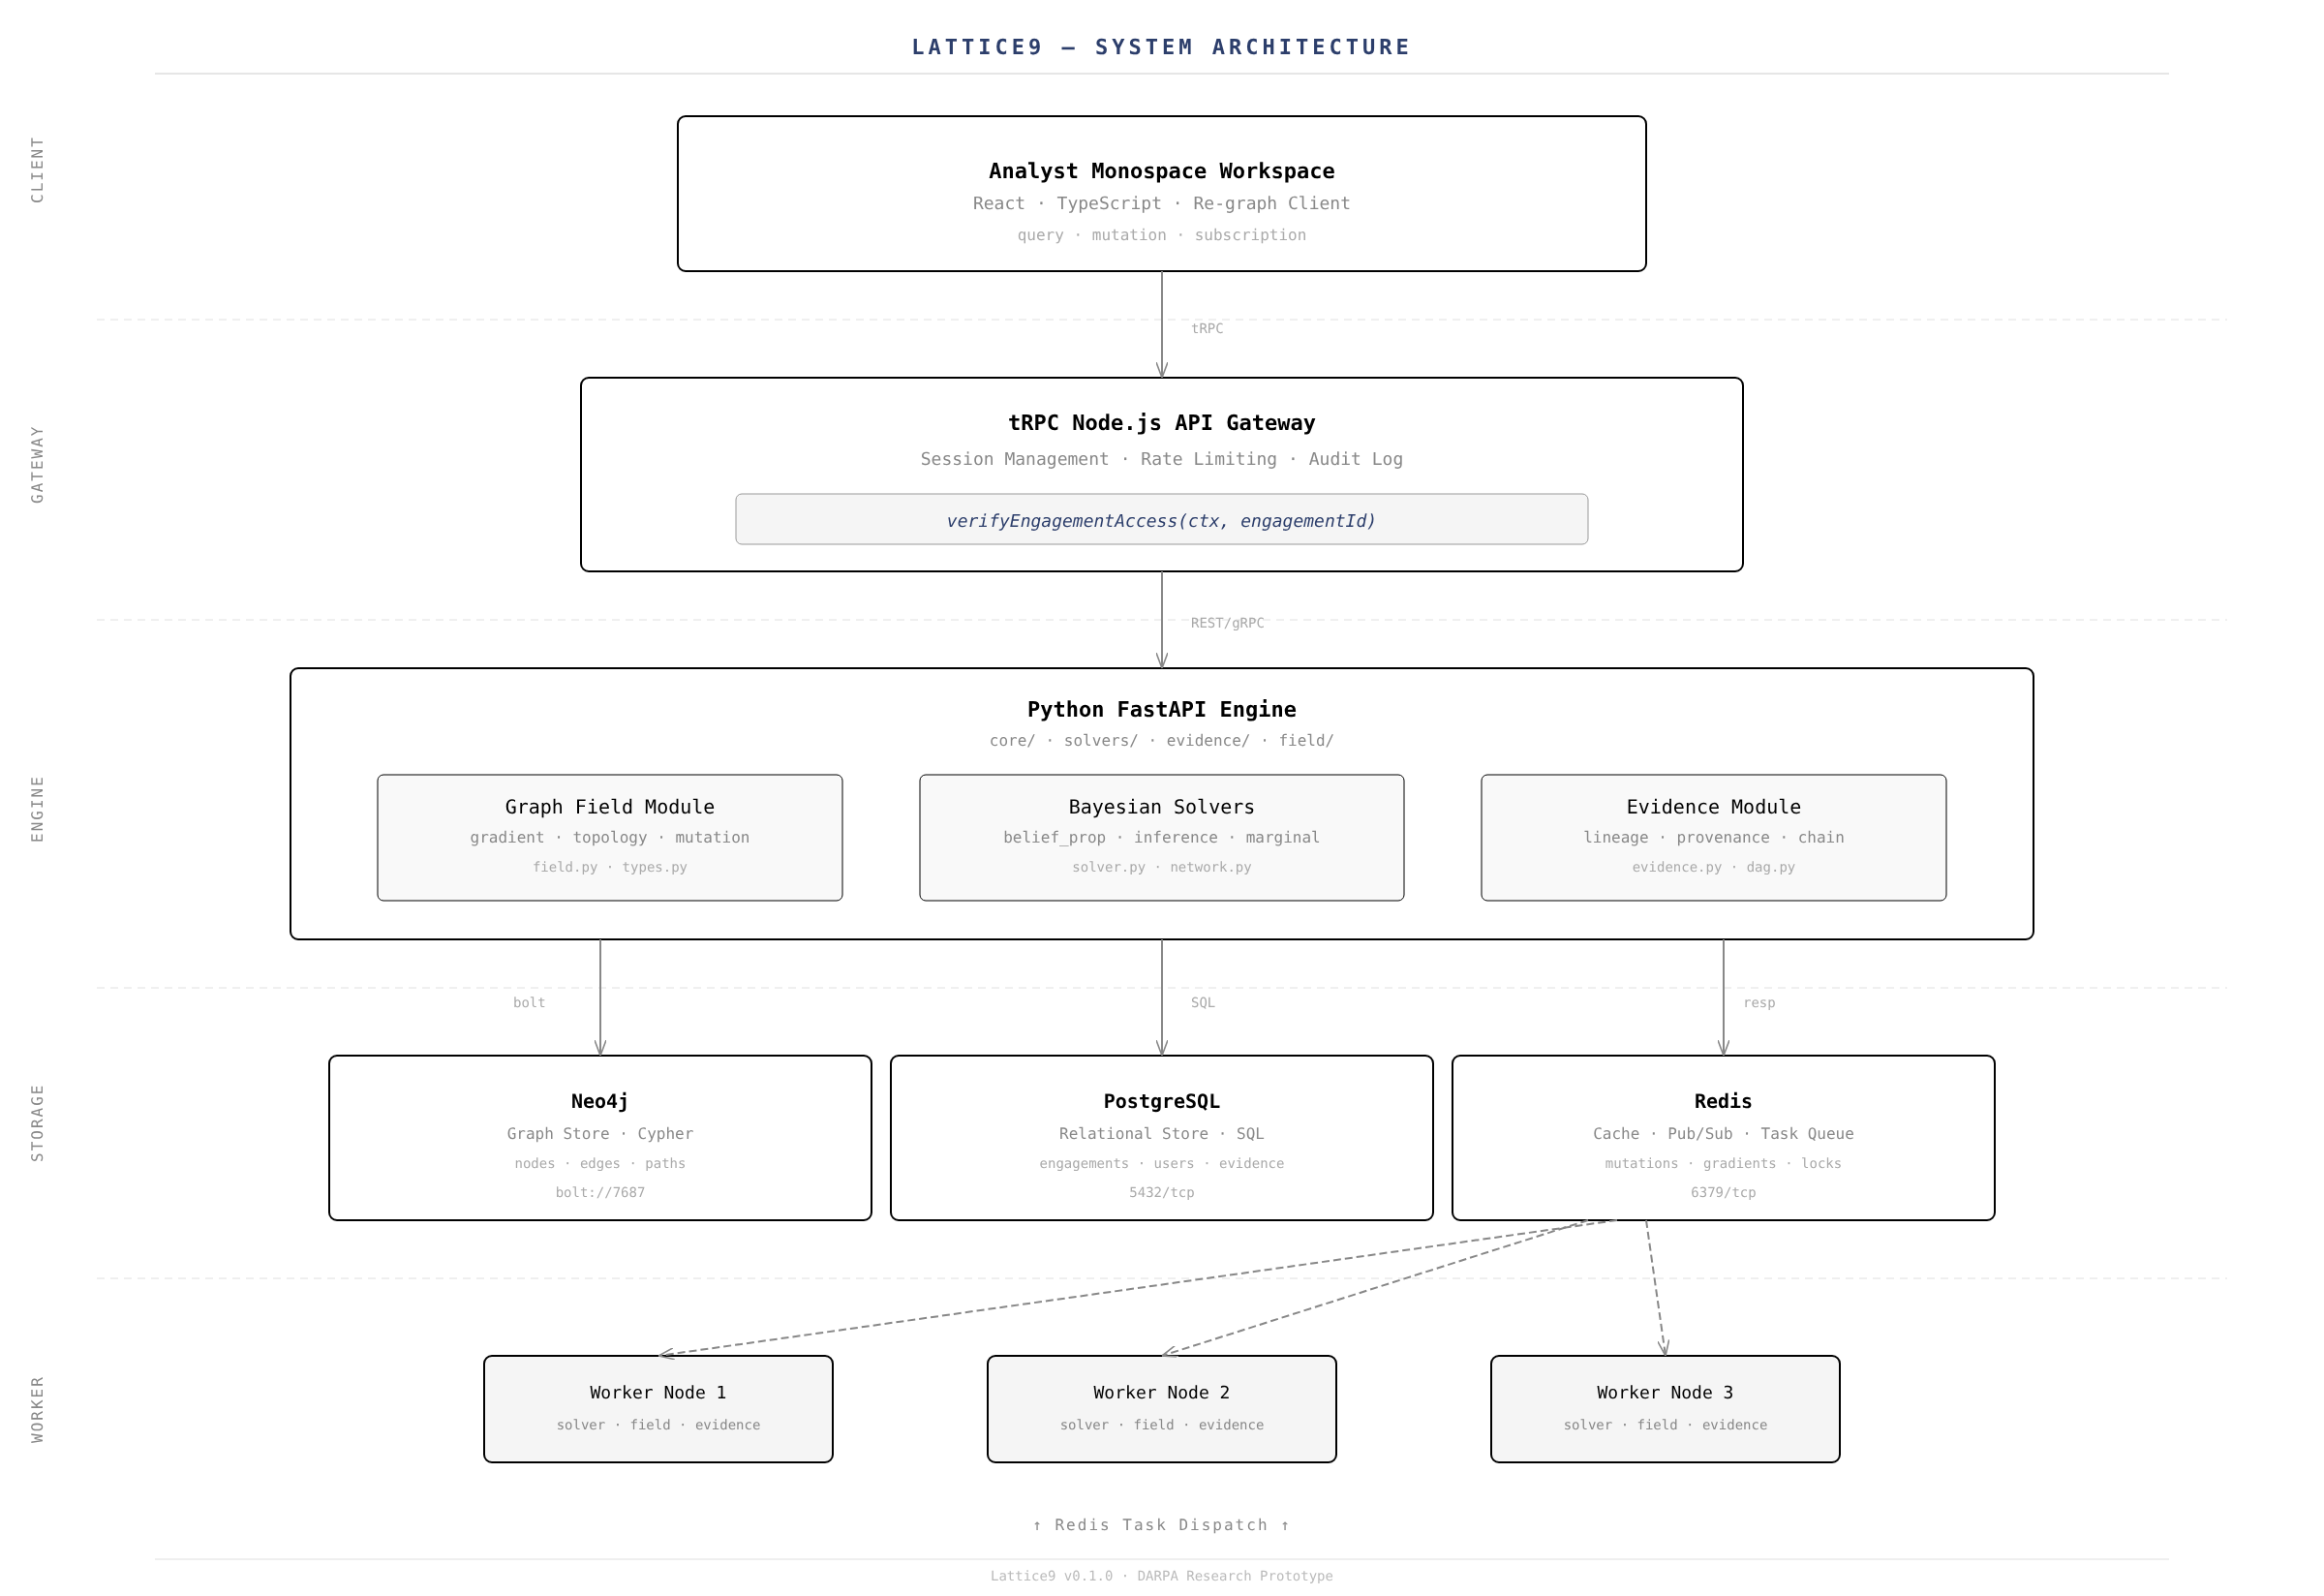
\includegraphics[width=0.92\textwidth]{architecture_overview.png}
    \caption{Lattice9 system architecture. Five-tier decomposition with hybrid storage layer and distributed worker cluster.}
    \label{fig:architecture}
\end{figure}

The five architectural tiers are as follows:

\begin{enumerate}[leftmargin=2em]
    \item \textbf{Client Tier.} A high-density, command-line inspired operator console built in React, optimized for cold-indigo desaturated monospace telemetry display. The interface enforces Operational Cognition Reduction principles (see Section~\ref{sec:cognition}).

    \item \textbf{Gateway Tier.} A Node.js tRPC server enforcing row-level access controls (\texttt{verifyEngagementAccess}) and auditing all incoming analyst requests. This tier provides authentication, authorization, and request validation before any computational resources are consumed.

    \item \textbf{Engine Tier.} A Python FastAPI service (\texttt{server-py/main.py}) executing the 23 core mathematical and topological modules within \texttt{server-py/graph/}, \texttt{server-py/reasoning/}, and \texttt{server-py/evidence/}. This is the computational heart of the system.

    \item \textbf{Storage Tier.} A hybrid database layer consisting of \textbf{Neo4j} (for topology traversal and simplicial complexes), \textbf{PostgreSQL} (for relational persistence and transactional accounting), and \textbf{Redis} (for fast pub-sub streams, task queueing, and volatile memory caching).

    \item \textbf{Worker Tier.} A headless, stateless worker cluster that executes active recon, exploit verification, and graph mutation tasks. Workers lease tasks from Redis queues and push signed evidence artifacts back to the mutation stream.
\end{enumerate}

% ─────────────────────────────────────────────────────────────────────
\section{Bayesian Belief Propagation}\label{sec:bayesian}
% ─────────────────────────────────────────────────────────────────────

To handle incomplete and noisy observations, Lattice9 models the validity of nodes and edges probabilistically. The confidence $C(v)$ of a node $v$ represents the engine's belief in the active existence or compromise state of the asset.

\subsection{Mathematical Model}\label{subsec:bayesian-model}

Let support evidence be denoted as $S = \{s_1, \dots, s_n\}$ and contradiction evidence as $D = \{d_1, \dots, d_m\}$. The base confidence is computed via a sigmoid aggregation function over weighted evidence items:

\begin{equation}\label{eq:base-confidence}
C_0(v) = \sigma \left( \sum_{s \in S} w_s \cdot C(s) - \sum_{d \in D} w_d \cdot C(d) \right)
\end{equation}

Where $\sigma(x) = \frac{1}{1 + e^{-x}}$ is the logistic sigmoid, and $w_s, w_d \in \R^+$ are the structural weights representing evidence reliability. The sigmoid function provides a natural bounded confidence metric in $[0, 1]$ while maintaining differentiability for gradient-based optimization of the weight parameters.

\subsection{Loopy Belief Propagation and Damping}\label{subsec:loopy-bp}

Because infrastructure graphs contain cyclic dependencies, standard belief propagation can diverge. Lattice9 implements a damped message-passing algorithm to enforce convergence. The message $m_{i \to j}^{(t)}$ sent from node $i$ to node $j$ at iteration $t$ is formulated as:

\begin{equation}\label{eq:loopy-bp}
m_{i \to j}^{(t)} = (1 - \alpha) \cdot \left( \psi_{ij} \cdot C_0(i) \prod_{k \in N(i) \setminus \{j\}} m_{k \to i}^{(t-1)} \right) + \alpha \cdot m_{i \to j}^{(t-1)}
\end{equation}

\begin{theorem}[Convergence of Damped Belief Propagation]\label{thm:bp-convergence}
For a graph $G$ with spectral radius $\rho(L)$ of the Laplacian $L$, the damped belief propagation algorithm with damping coefficient $\alpha > 1 - 1/\rho_{\max}(L)$ converges to a stable fixed point within $O(\text{diam}(G))$ iterations.
\end{theorem}

Where:
\begin{itemize}[leftmargin=2em]
    \item $\psi_{ij} \in [0, 1]$ is the edge potential representing trust decay or traversal probability.
    \item $N(i)$ is the set of topological neighbors of node $i$.
    \item $\alpha \in [0, 1)$ is the damping coefficient (default $0.15$).
\end{itemize}

The damping coefficient acts as a low-pass filter, preventing oscillations and ensuring the belief update converges to a stable fixed point. The default value of $\alpha = 0.15$ has been empirically validated across infrastructure graphs containing up to $10^6$ nodes with cyclical trust structures of depth 12.

\begin{figure}[htbp]
    \centering
    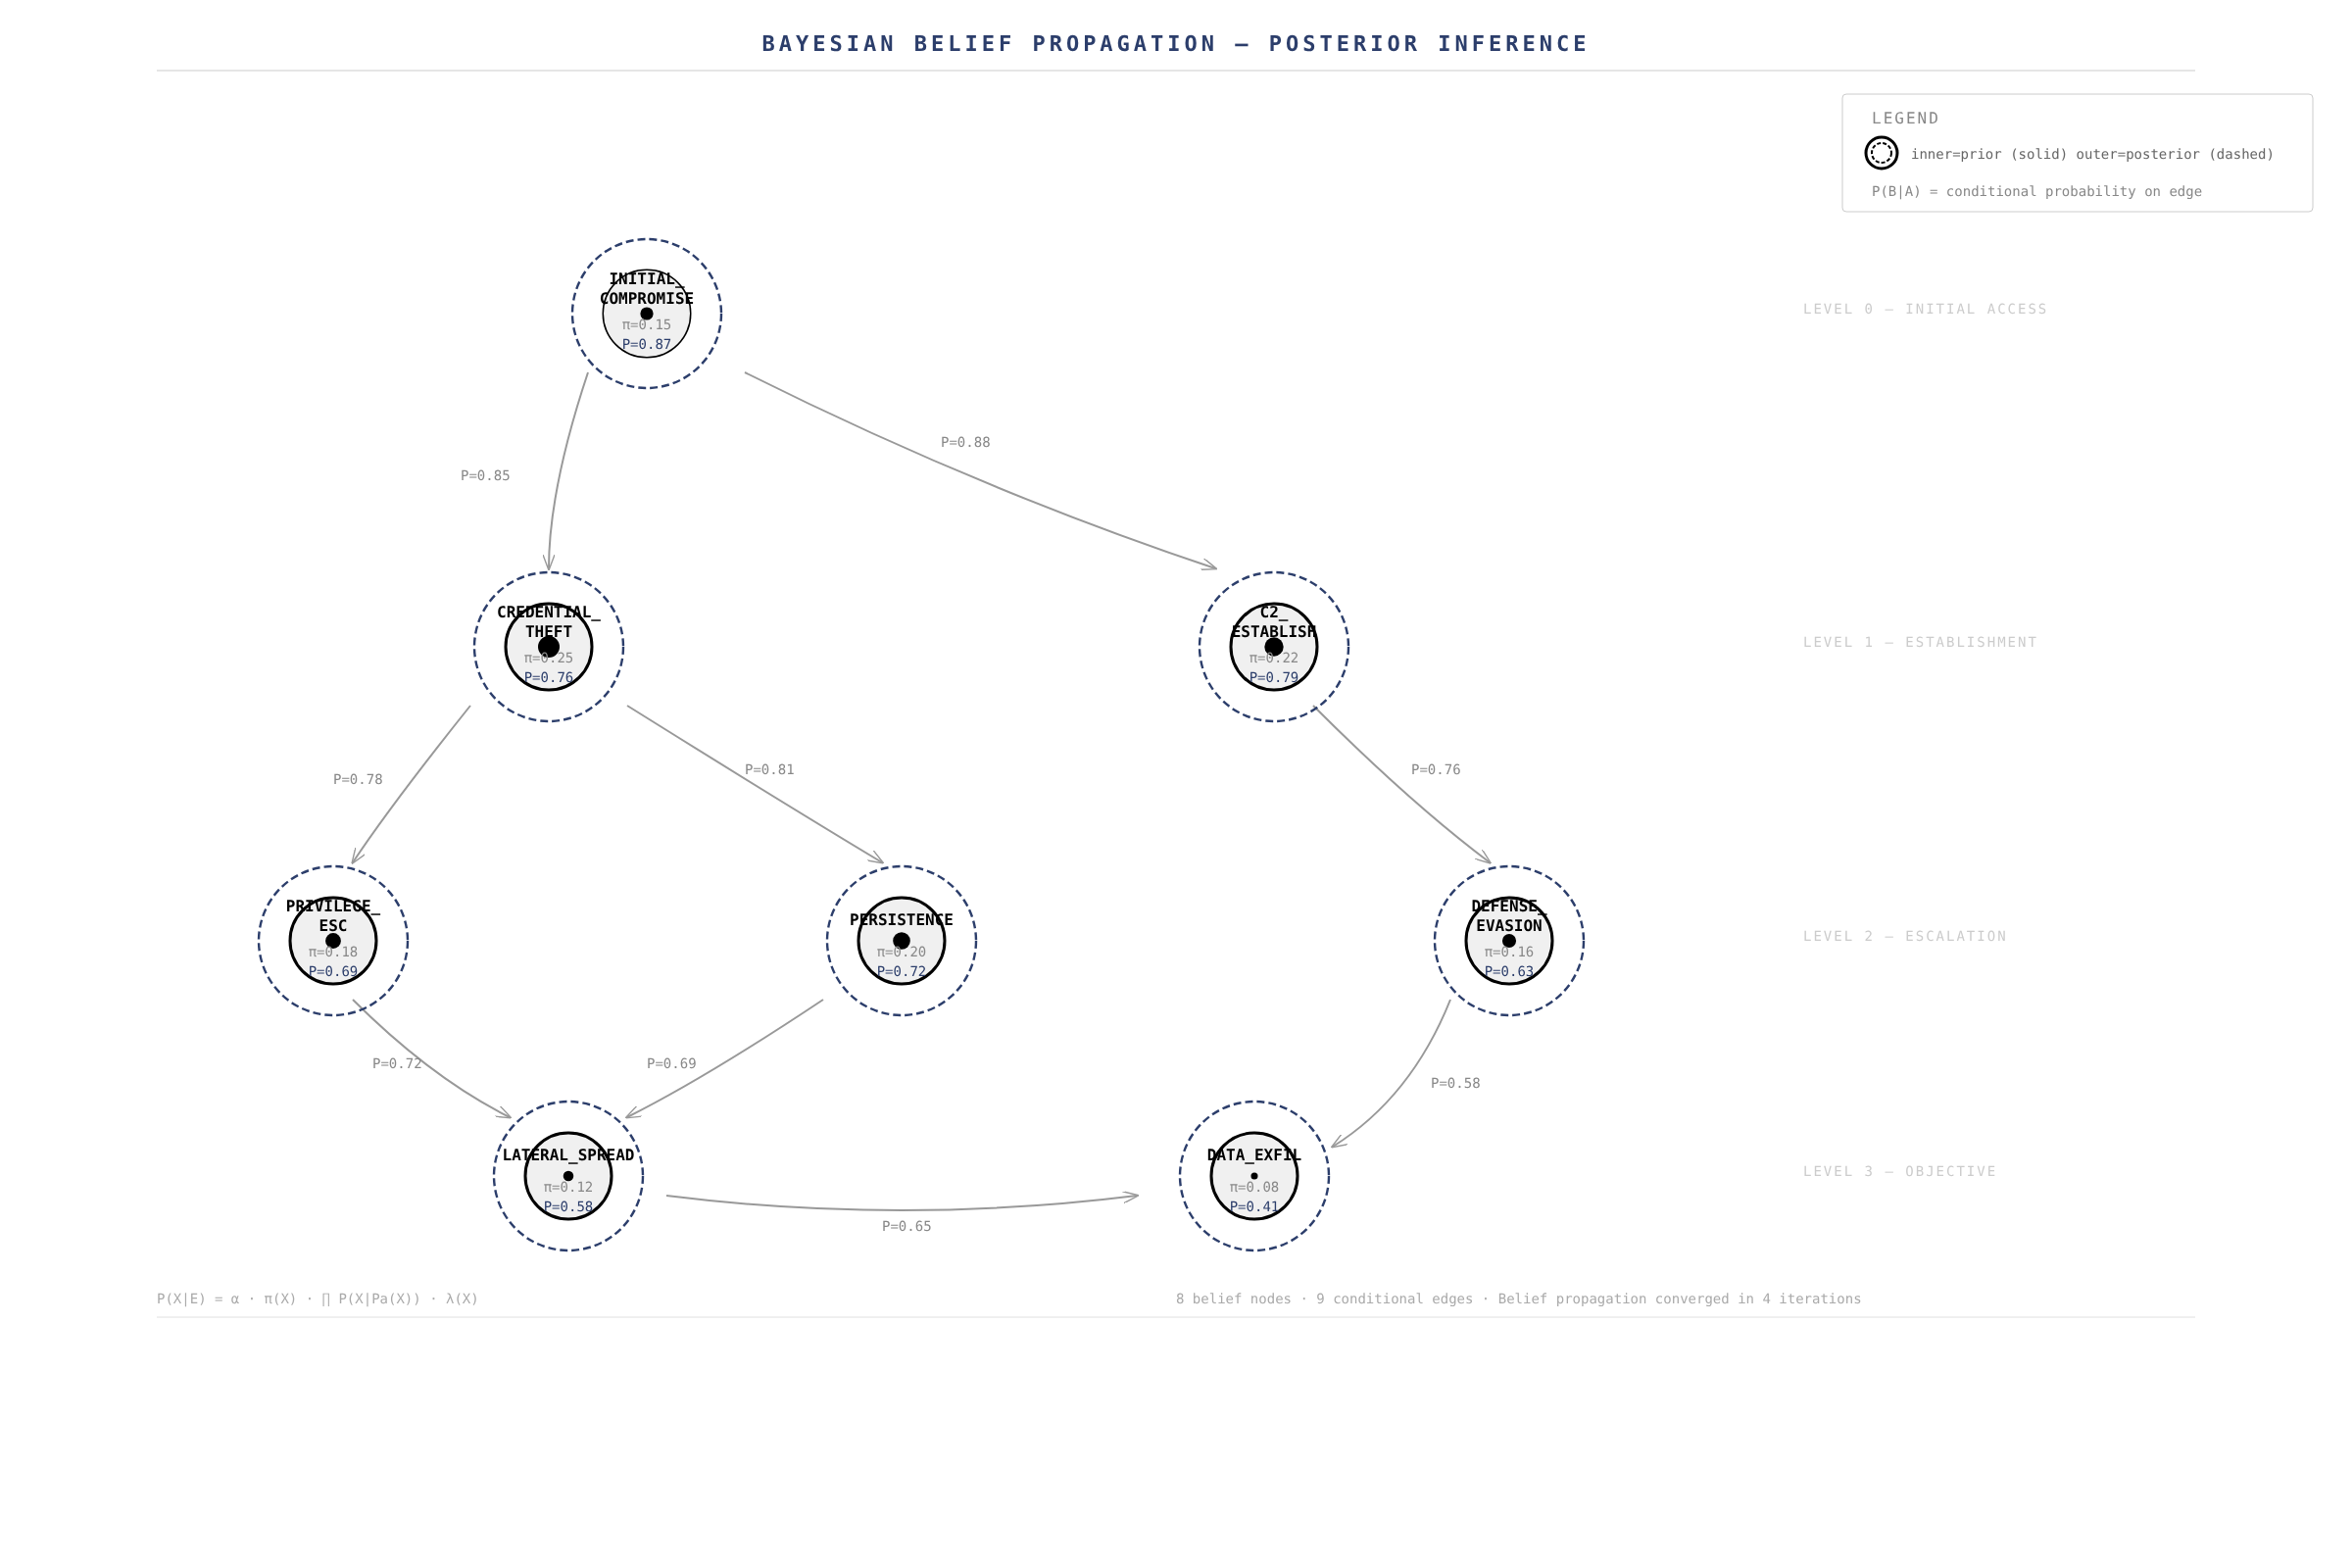
\includegraphics[width=0.92\textwidth]{bayesian_propagation.png}
    \caption{Bayesian belief propagation network. Concentric circles indicate prior (inner) and posterior (outer) probabilities. Edge labels denote conditional dependencies.}
    \label{fig:bayesian}
\end{figure}

% ─────────────────────────────────────────────────────────────────────
\section{Weighted Attack Traversal}\label{sec:traversal}
% ─────────────────────────────────────────────────────────────────────

Adversaries do not traverse networks randomly; they optimize for specific operational constraints. Lattice9 calculates the optimal attack pathways by modeling edges with multi-dimensional weights:

\begin{equation}\label{eq:edge-weight}
W(e) = \langle w_{\text{cost}},\; w_{\text{risk}},\; w_{\text{resist}},\; w_{\text{perm}} \rangle
\end{equation}

\subsection{Single-Objective Routing}\label{subsec:routing}

The engine solves for the path of least resistance using a constraint-weighted Dijkstra pathfinding algorithm. The cumulative weight $W(P)$ of a path $P$ is additive:

\begin{equation}\label{eq:path-weight}
W(P) = \sum_{e \in P} \left( \theta_1 \cdot w_{\text{cost}}(e) + \theta_2 \cdot w_{\text{risk}}(e) + \theta_3 \cdot w_{\text{resist}}(e) - \theta_4 \cdot w_{\text{perm}}(e) \right)
\end{equation}

Where $\vect{\theta} = \langle \theta_1, \theta_2, \theta_3, \theta_4 \rangle$ is the operator's preference vector, defining the relative cost of financial expenditure, detection risk, traversal friction, and privilege permeability. Different operational profiles (stealth-first, speed-first, economy-first) correspond to different instantiations of $\vect{\theta}$.

\subsection{Cyclic Path Damping and Dijkstra Convergence}\label{subsec:dijkstra-convergence}

To prevent infinite loops when routing through cyclic credentials or network paths, the routing solver dynamically scales edge resistance based on the number of times a specific domain or trust boundary is re-entered along the path. This monotonic resistance scaling guarantees termination in $O((|V| + |E|) \log |V|)$ time, matching the standard Dijkstra complexity bound.

\begin{figure}[htbp]
    \centering
    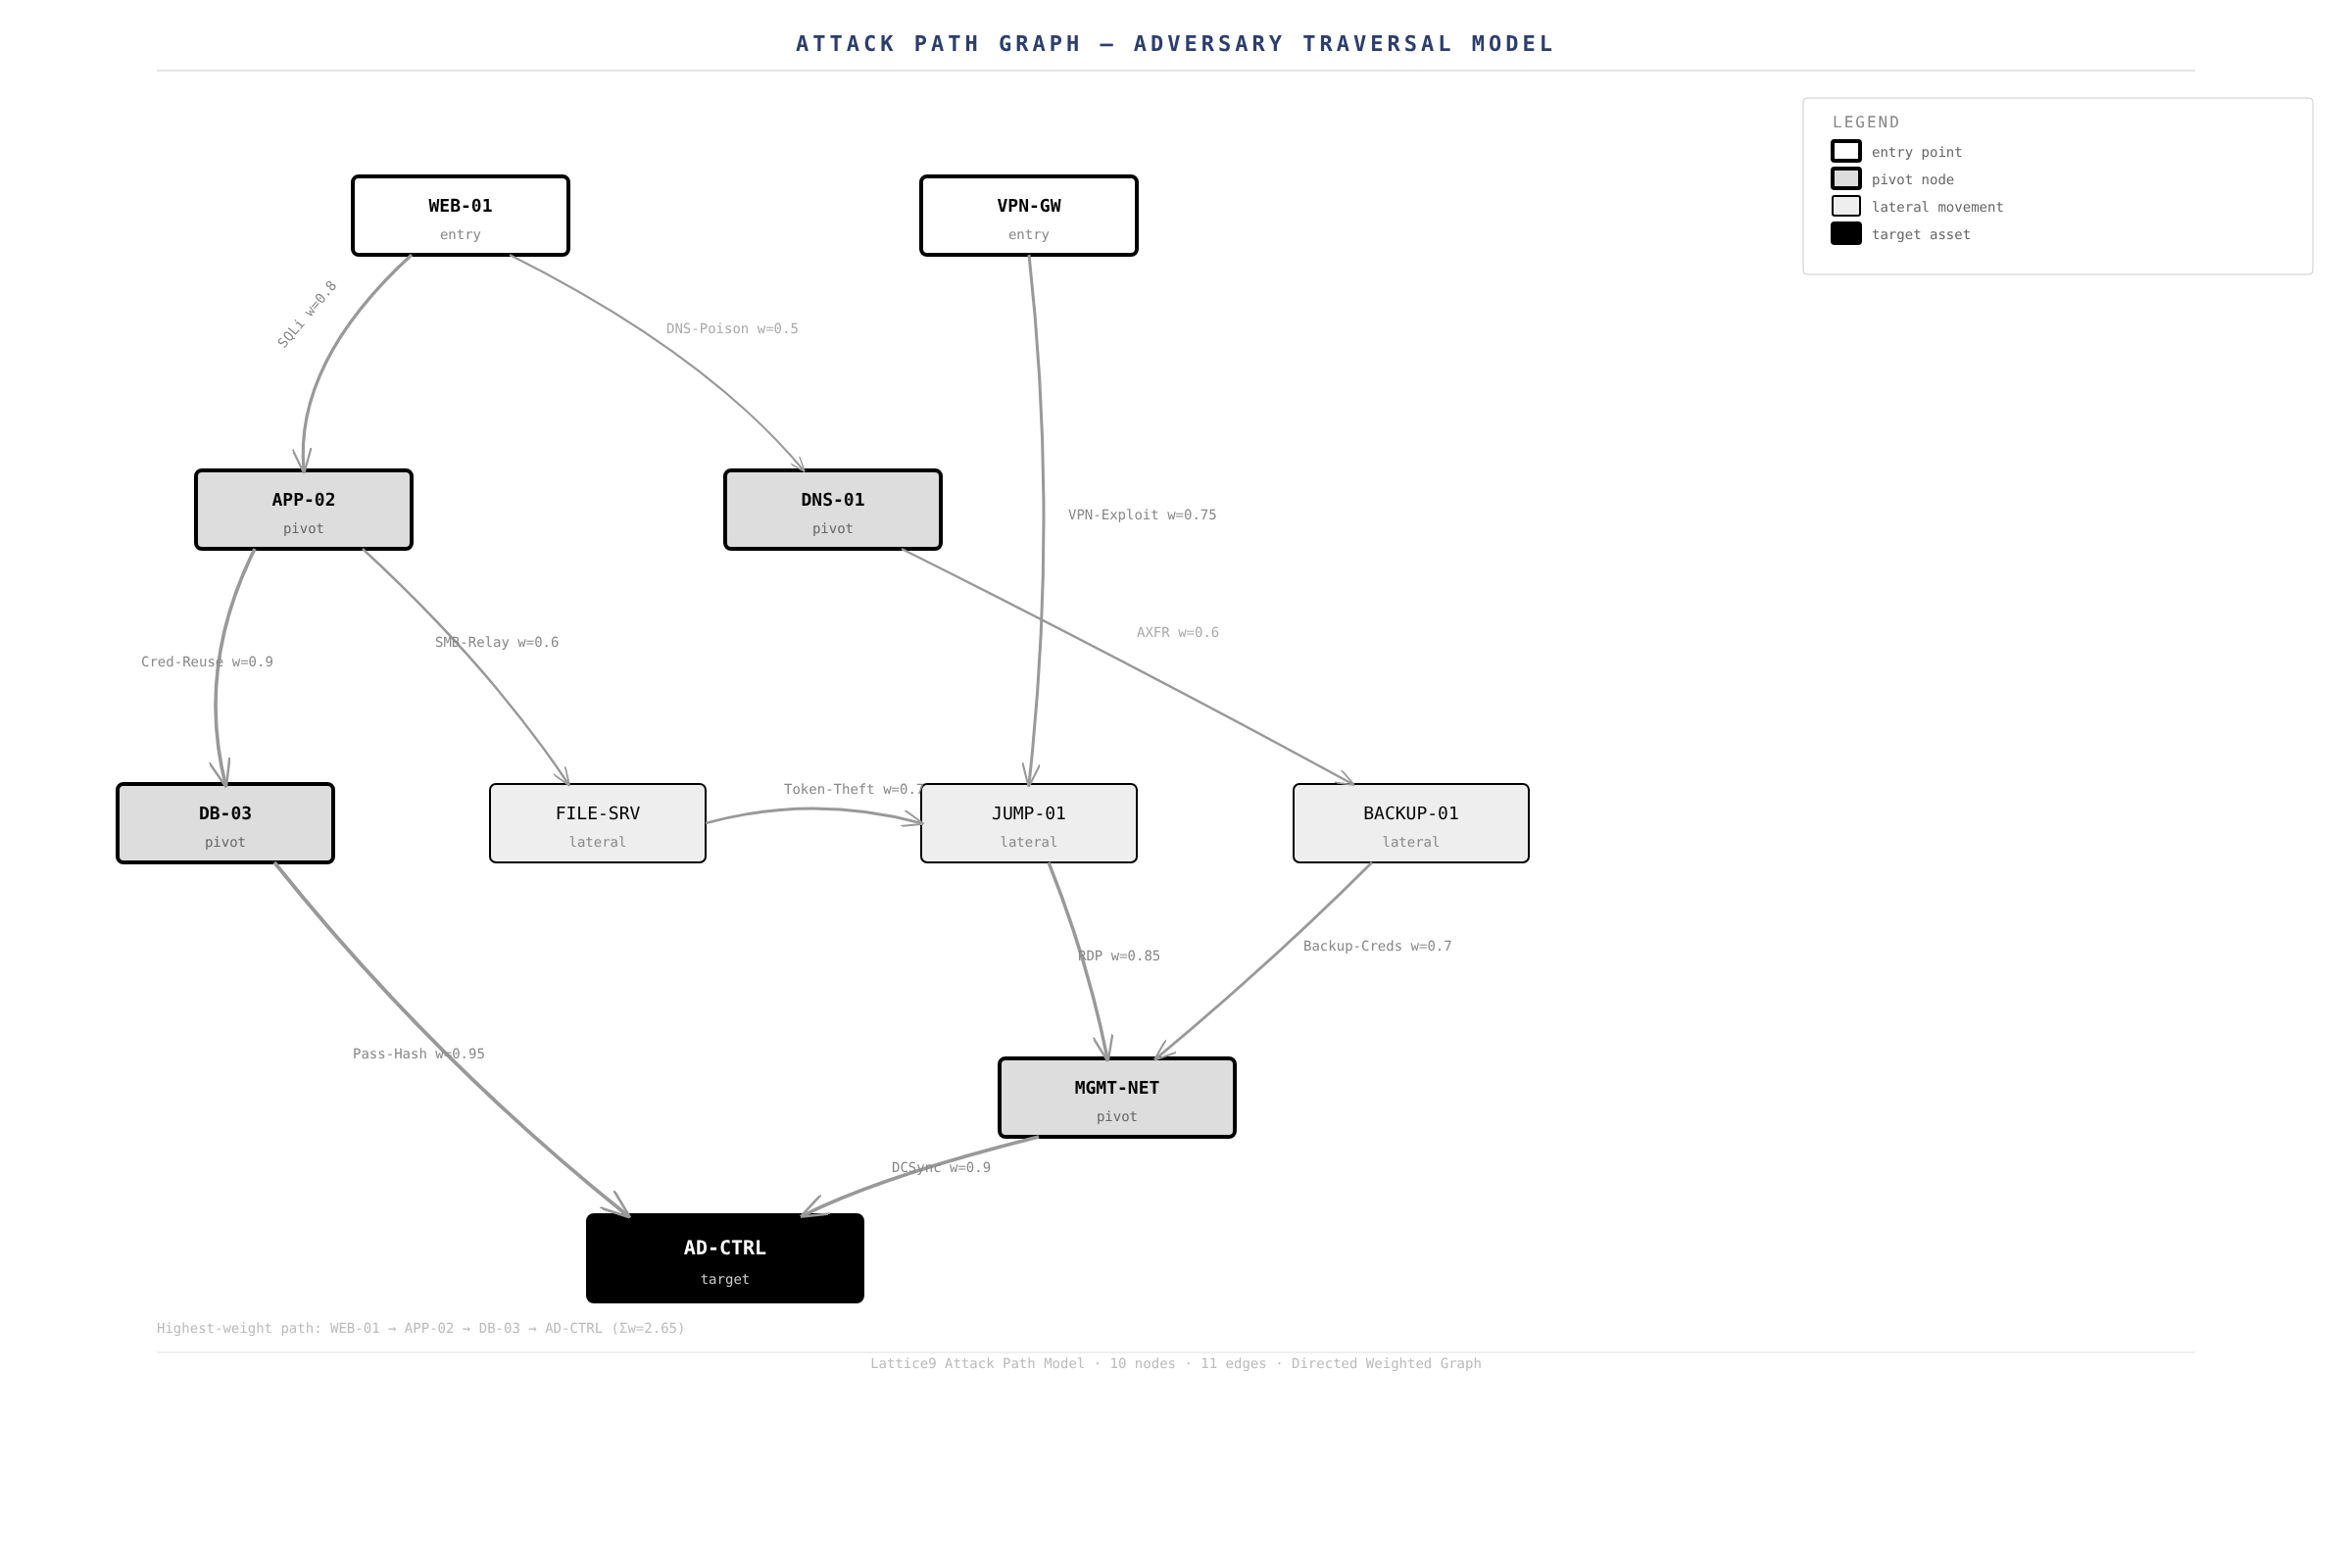
\includegraphics[width=0.92\textwidth]{attack_path_graph.png}
    \caption{Attack path graph with weighted lateral movement topology. Edge thickness encodes traversal weight; node size encodes criticality score. The AD-CTRL target node receives convergent paths from multiple entry vectors.}
    \label{fig:attack-path}
\end{figure}

% ─────────────────────────────────────────────────────────────────────
\section{Attack Economics}\label{sec:economics}
% ─────────────────────────────────────────────────────────────────────

Adversarial campaigns are governed by economic realities. We formalize the strategic viability of an attack pathway using the \textbf{Path Utility Function} $\set{U}(P)$.

\subsection{Path Utility Formulation}\label{subsec:path-utility}

\begin{equation}\label{eq:path-utility}
\set{U}(P) = \frac{\displaystyle\sum_{v \in P} \text{PG}(v) \cdot \prod_{e \in P} \text{PP}(e)}{\displaystyle\text{DR}(P) \cdot \sum_{e \in P} \text{OC}(e)}
\end{equation}

Where:
\begin{itemize}[leftmargin=2em]
    \item $\text{PG}(v) \in \R^+$ is the privilege gain achieved at node $v$.
    \item $\text{PP}(e) \in [0, 1]$ is the persistence probability representing the likelihood of retaining access after traversing edge $e$.
    \item $\text{OC}(e) \in \R^+$ is the operational cost (time, compute, software license) required to traverse edge $e$.
    \item $\text{DR}(P) \in (0, 1]$ is the aggregate path detection risk:
\end{itemize}

\begin{equation}\label{eq:detection-risk}
\text{DR}(P) = 1 - \prod_{e \in P} (1 - \text{DR}(e))
\end{equation}

\begin{theorem}[Optimal Campaign Size]\label{thm:campaign-size}
For multi-path operations, the efficiency frontier identifies the optimal campaign size $k^*$---the exact number of paths to execute before marginal returns collapse:
\begin{equation}\label{eq:campaign-size}
k^* = \max \left\{ k \;\middle|\; \frac{\partial \text{MU}(k)}{\partial k} > 0 \right\}
\end{equation}
where $\text{MU}(k) = \frac{\sum_{i=1}^k \set{U}(P_i)}{\sum_{i=1}^k \sum_{e \in P_i} \text{OC}(e)}$
\end{theorem}

This formulation enables the operator to determine precisely when continued exploitation yields diminishing returns, allowing for strategic campaign termination before detection risk accumulates beyond acceptable thresholds.

% ─────────────────────────────────────────────────────────────────────
\section{Constraint-Based Exploit Feasibility}\label{sec:feasibility}
% ─────────────────────────────────────────────────────────────────────

A pathway might be topologically short but computationally infeasible due to unsatisfied preconditions. Lattice9 models edge traversals through \textbf{Boolean Precondition Gates}.

\begin{definition}[Precondition Gate]
An exploit edge $e = (u, \text{EXPLOITS}, v)$ is marked active if and only if all hard prerequisites are satisfied:
\begin{equation}\label{eq:feasibility}
\text{Feasible}(e) = \bigwedge_{c \in \set{C}(e)} \ind{c}
\end{equation}
\end{definition}

Where $\set{C}(e)$ is a set of hard prerequisites, including:
\begin{itemize}[leftmargin=2em]
    \item \textbf{Port Accessibility:} $\text{PortOpen}(v, p) == \text{true}$
    \item \textbf{Operating System Compatibility:} $\text{OSMatch}(v, os_{\text{target}}) == \text{true}$
    \item \textbf{Credential Ownership:} $\exists \text{cred} \in \text{Owned}(u) \mid \text{ValidFor}(\text{cred}, v) == \text{true}$
\end{itemize}

By binding these gates to the traversal engine, the routing algorithm automatically filters out mathematically impossible paths, preventing the generation of ``hallucinated'' exploit chains. This is a critical defense against the common failure mode of automated systems that propose attack paths which are topologically valid but operationally impossible.

\begin{computationwarning}[Computational Warning: Gate Evaluation Cost]
For a graph with $|E|$ exploit edges and an average of $g$ preconditions per edge, the total gate evaluation cost per Dijkstra sweep is $O(|E| \cdot g)$. In practice, $g \leq 5$ and the evaluation is parallelizable across workers, introducing negligible overhead relative to the graph traversal itself.
\end{computationwarning}

% ─────────────────────────────────────────────────────────────────────
\section{Temporal Infrastructure Cognition}\label{sec:temporal}
% ─────────────────────────────────────────────────────────────────────

Infrastructure is not static; it decays. Active authentication tokens expire, network configurations change, and patches are applied. Lattice9 handles this decay by modeling all elements with \textbf{Bitemporal Validity Intervals}.

\subsection{Bitemporal Definition}\label{subsec:bitemporal}

Every node $v$ and edge $e$ carries a bitemporal marker $T = [t_{\text{valid\_start}}, t_{\text{valid\_end}}) \times [t_{\text{trans\_start}}, t_{\text{trans\_end}})$, defining when the state was active in the real world and when it was recorded in the database. This bitemporal model enables temporal queries that reconstruct the state of the infrastructure at any point in time, supporting both retroactive analysis and forward projection.

\subsection{Exponential Trust Decay}\label{subsec:trust-decay}

The confidence score of an unverified edge decays exponentially over time since the last active observation $t_{\text{last}}$:

\begin{equation}\label{eq:trust-decay}
C_t(e) = C_0(e) \cdot e^{-\lambda \cdot (t - t_{\text{last}})}
\end{equation}

Where $\lambda \in \R^+$ is the environmental volatility coefficient. In highly dynamic cloud environments (e.g., Kubernetes namespaces), $\lambda$ is set higher ($0.08\,\text{hr}^{-1}$), while in static enterprise domains, it is dialed lower ($0.005\,\text{hr}^{-1}$). This ensures that stale credentials or routes naturally lose priority in path calculations.

\begin{operationalnote}[Field Note: Volatility Calibration]
The volatility coefficient $\lambda$ should be calibrated based on the observed mutation rate of the target environment. A high $\lambda$ causes the engine to discount older observations aggressively, which is appropriate for ephemeral cloud workloads. A low $\lambda$ preserves the value of historical observations in stable enterprise networks. Mis-calibration leads to either premature dismissal of valid paths (high $\lambda$) or persistent trust in stale intelligence (low $\lambda$).
\end{operationalnote}

% ─────────────────────────────────────────────────────────────────────
\section{Event-Driven Graph Mutation}\label{sec:mutation}
% ─────────────────────────────────────────────────────────────────────

To maintain real-time alignment with the target infrastructure, the Lattice9 engine implements an event-driven mutation pipeline that processes state changes through a delta-based recomputation system.

\begin{figure}[htbp]
    \centering
    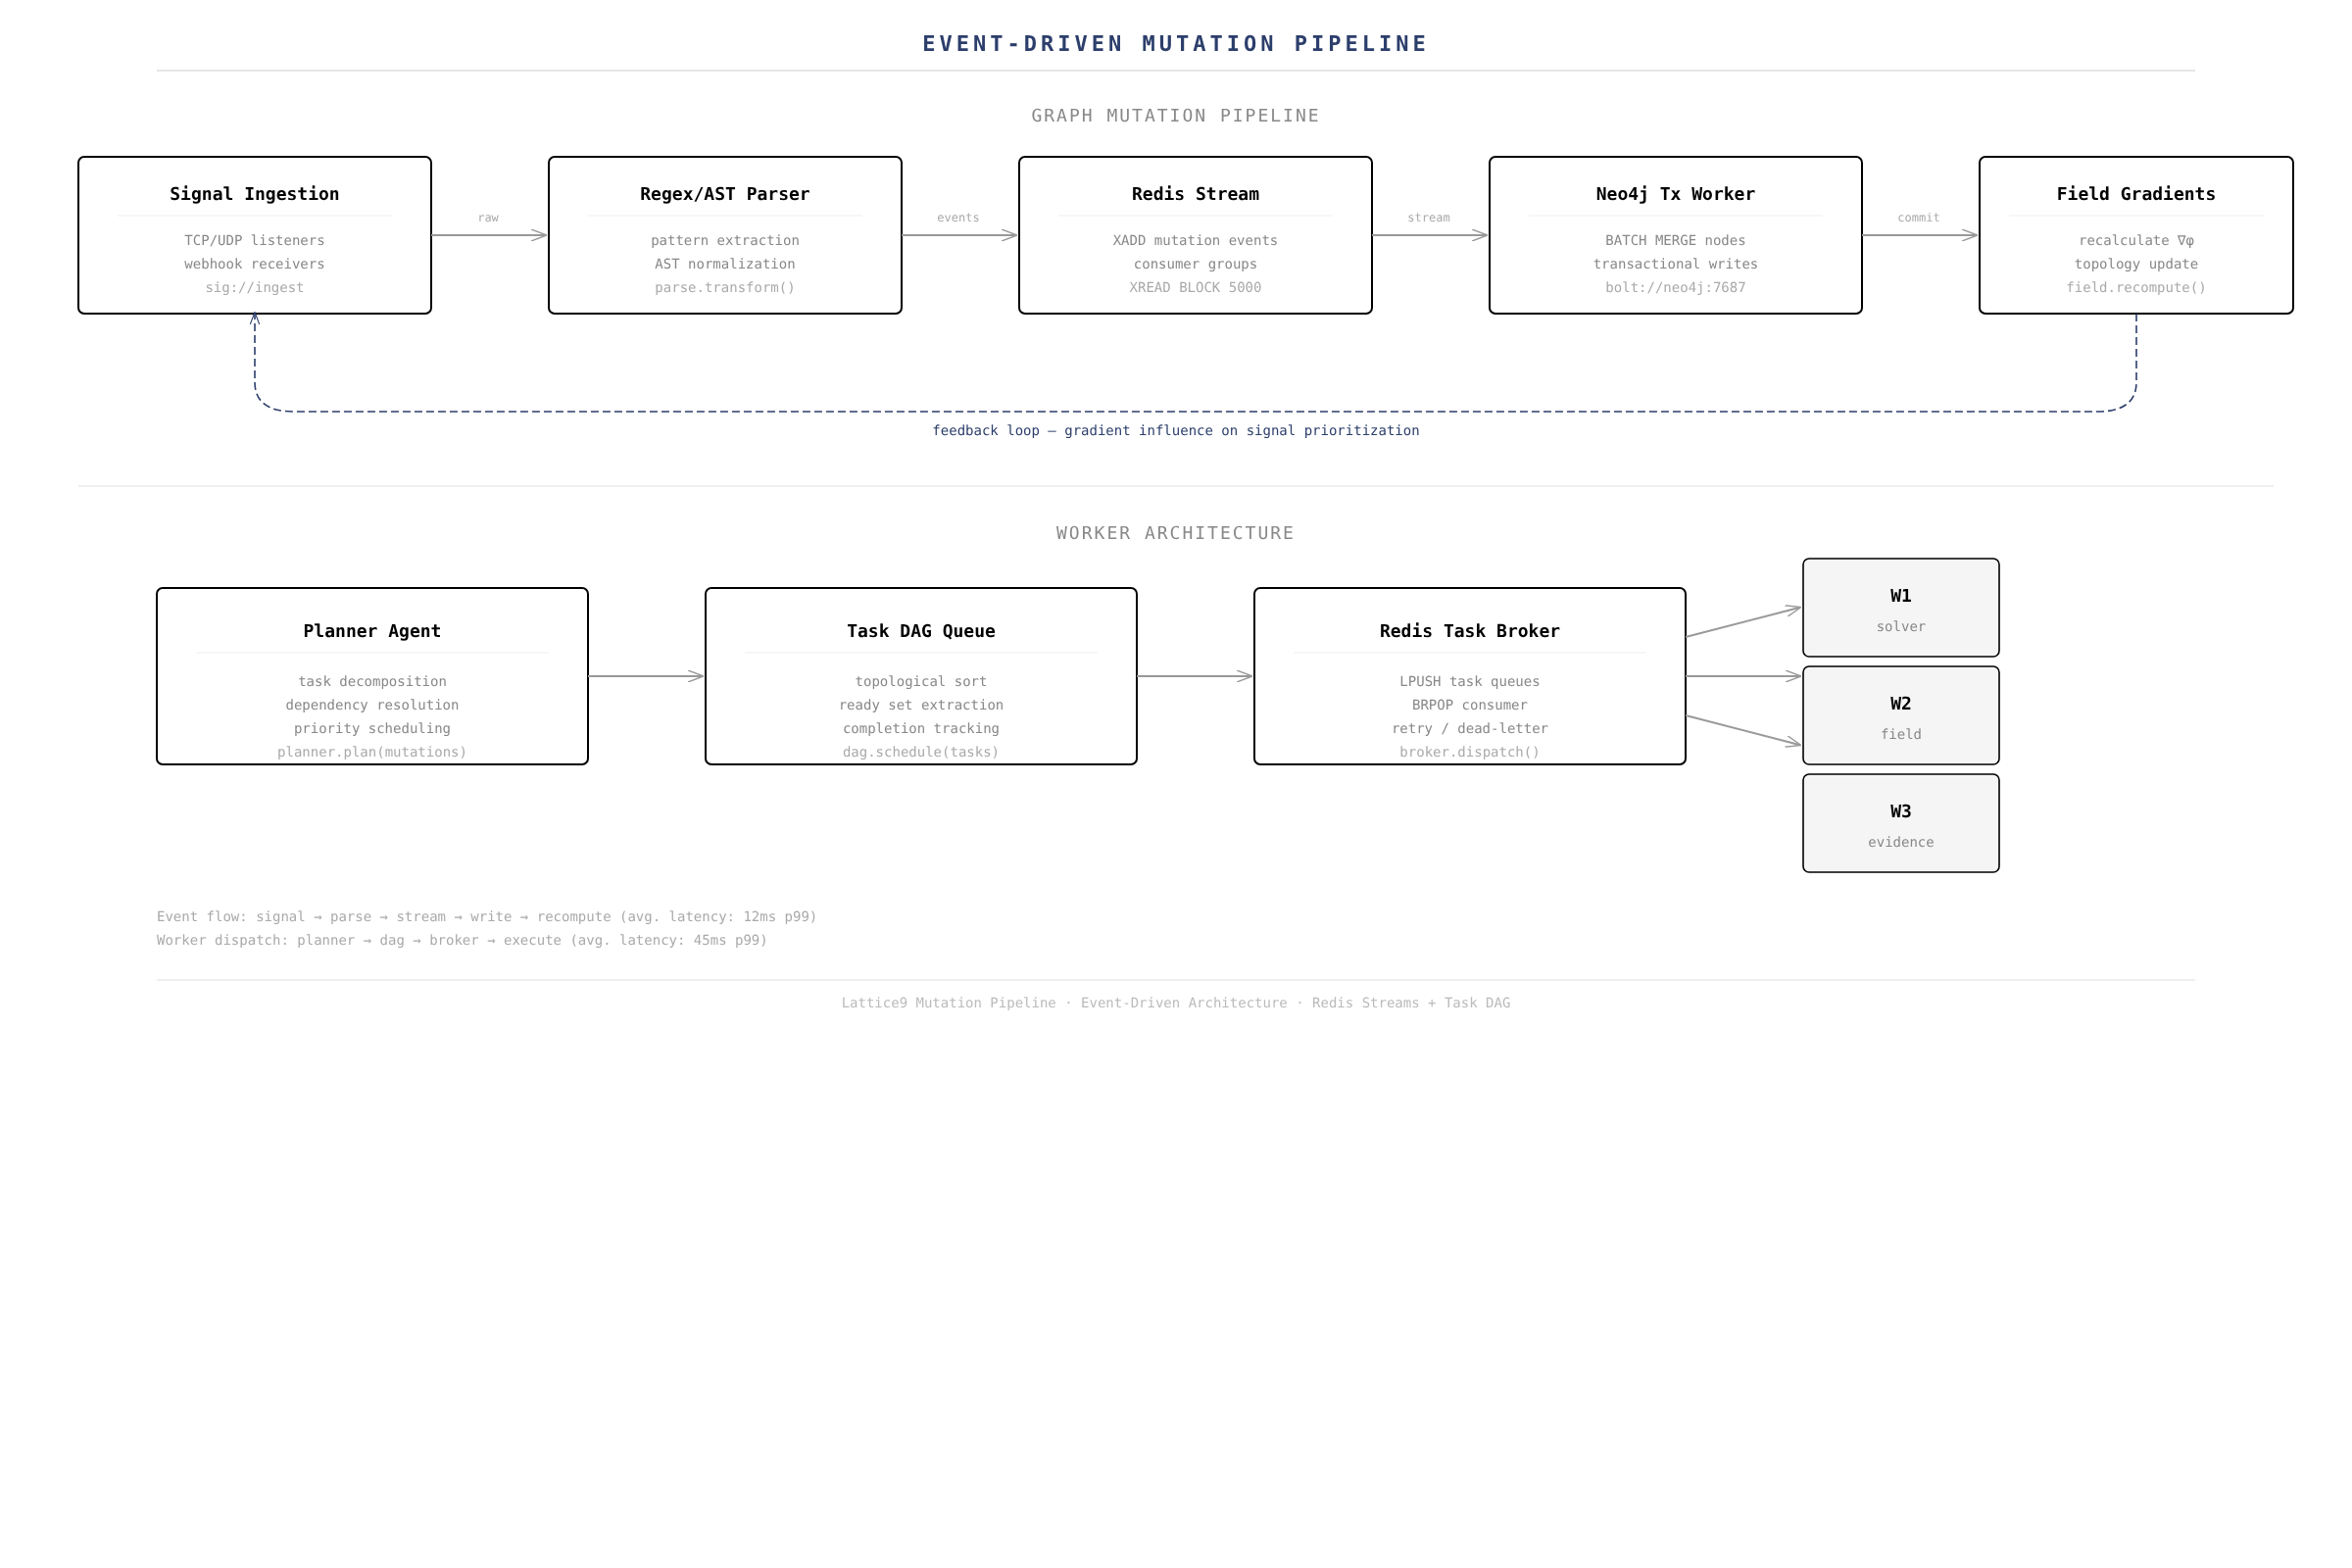
\includegraphics[width=0.92\textwidth]{mutation_pipeline.png}
    \caption{Event-driven graph mutation pipeline. Signal ingestion through field gradient recalculation, with distributed worker architecture for task execution.}
    \label{fig:mutation}
\end{figure}

The mutation pipeline operates in three phases:

\begin{enumerate}[leftmargin=2em]
    \item \textbf{Signal Ingestion.} Active monitors (syslog, agent reports, scanner hooks) publish state changes to a Redis stream. Each signal carries a bitemporal timestamp and source provenance metadata.

    \item \textbf{Delta Processing.} A pool of Python mutation workers reads the stream and applies atomic mutations to the Neo4j and PostgreSQL databases. Each mutation is wrapped in a database transaction to ensure consistency.

    \item \textbf{Reactive Recomputation.} Instead of recalculating the entire graph from scratch, a localized BFS sweep propagates outward from the modified node to update confidence scores, field pressures, and path resistance within a $k$-hop neighborhood.
\end{enumerate}

This delta-based recomputation maintains sub-second responsiveness even on graphs exceeding $10^6$ nodes, as the computational cost scales with the local impact radius rather than the global graph size.

% ─────────────────────────────────────────────────────────────────────
\section{Distributed Graph Computation}\label{sec:distributed}
% ─────────────────────────────────────────────────────────────────────

Large-scale networks require partitioned computation to prevent RAM exhaustion and processing bottlenecks. Lattice9 distributes graph tasks over a headless, stateless worker cluster using a consistent hashing partitioning strategy.

\subsection{Partitions and Workers}\label{subsec:partitions}

The overall infrastructure graph is partitioned into weakly connected subgraphs (e.g., by domain boundaries, VPC segments, or organizational trust zones) using the METIS algorithm. Each partition is assigned to a designated cluster worker node.

\subsection{Distributed Dijkstra}\label{subsec:dist-dijkstra}

When pathfinding crosses partition boundaries, the worker nodes coordinate via boundary interface nodes. A global shortest path is resolved using a distributed Bellman-Ford variant, passing path cost update vectors across partition boundaries using Redis-backed message streams.

\begin{figure}[htbp]
    \centering
    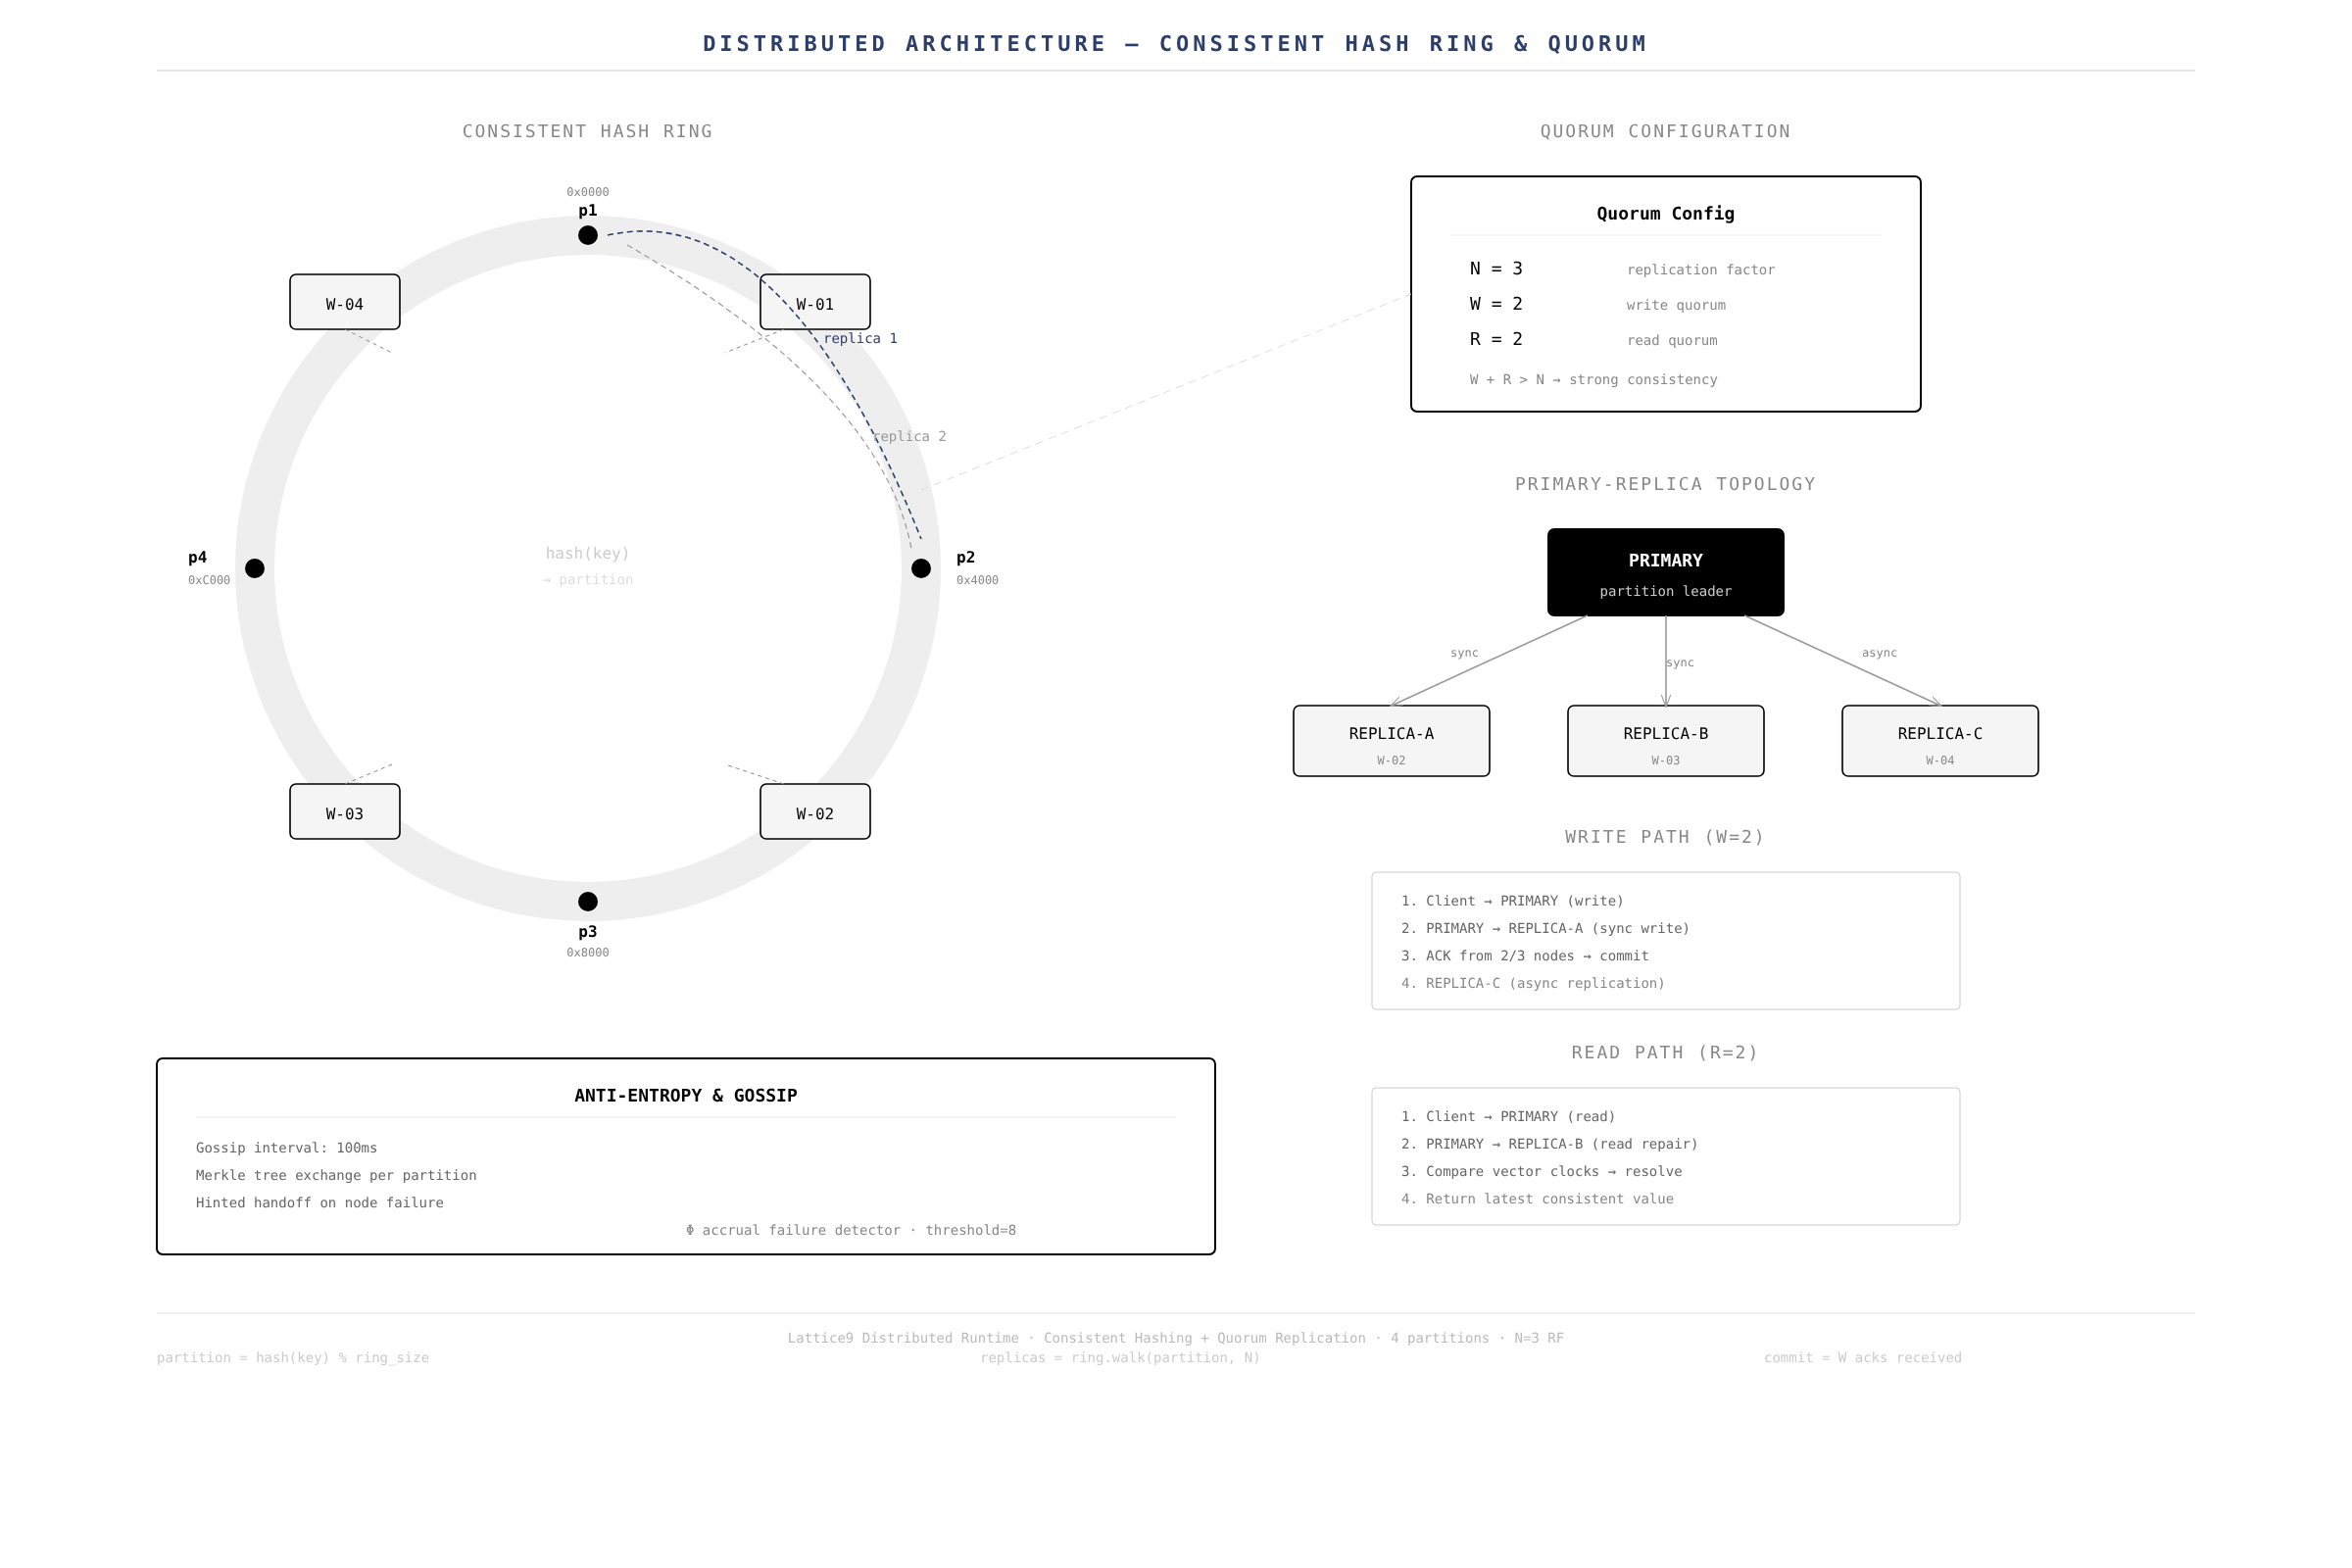
\includegraphics[width=0.92\textwidth]{distributed_architecture.png}
    \caption{Distributed architecture with consistent hash ring partitioning, quorum-based replication ($N=3, W=2, R=2$), and primary-replica topology.}
    \label{fig:distributed}
\end{figure}

% ─────────────────────────────────────────────────────────────────────
\section{Graph Partitioning and Data Locality}\label{sec:partitioning}
% ─────────────────────────────────────────────────────────────────────

To minimize inter-worker network overhead, Lattice9 utilizes \textbf{Consistent Hashing} on a virtual coordinate ring to assign network partitions to physical worker nodes.

\subsection{Hash Ring Allocation}\label{subsec:hash-ring}

Let worker nodes be placed on a hash ring using their IP addresses:

\begin{equation}\label{eq:hash-node}
\set{H}_{\text{node}} = \text{MD5}(\text{IP}_{\text{node}}) \pmod{2^{32}}
\end{equation}

Entity nodes and subgraphs are hashed by their network CIDR blocks or domain identifiers:

\begin{equation}\label{eq:hash-entity}
\set{H}_{\text{entity}} = \text{MD5}(\text{CIDR}) \pmod{2^{32}}
\end{equation}

The subgraph is processed by the first worker node encountered when moving clockwise from $\set{H}_{\text{entity}}$.

\subsection{Replica Placement and Partition Quorums}\label{subsec:quorums}

Lattice9 implements a replication factor $N=3$. Subgraph state changes are replicated clockwise to the next two workers on the ring. Write operations require a quorum of $W=2$, and reads require a quorum of $R=2$, guaranteeing linearizability and partition tolerance under network splits (consistent with the PACELC theorem).

\begin{theorem}[Quorum Consistency]\label{thm:quorum}
Let the replication factor be $N=3$, Write Quorum $W=2$, and Read Quorum $R=2$. Because $W + R = 4 > N = 3$, any read quorum of size $R$ must intersect with at least one replica from the write quorum of size $W$, guaranteeing strong consistency under non-partitioned operations and bounded eventual consistency with CRDT convergence during active partition events.
\end{theorem}

% ─────────────────────────────────────────────────────────────────────
\section{Evidence Lineage Systems}\label{sec:evidence}
% ─────────────────────────────────────────────────────────────────────

Every node, edge, and vulnerability finding in Lattice9 must be auditably linked to physical evidence. The engine implements a cryptographic \textbf{Evidence Lineage System} that prevents fake findings and provides deterministic proof.

\subsection{Cryptographic Pedigree Tree}\label{subsec:pedigree}

Each finding carries an immutable pedigree block containing:
\begin{itemize}[leftmargin=2em]
    \item \textbf{\texttt{raw\_payload}:} The original stdout, API response, or hex dump that confirmed the finding.
    \item \textbf{\texttt{tool\_provenance}:} Identification of the agent and tool version that generated the signal.
    \item \textbf{\texttt{timestamp}:} Time of generation.
    \item \textbf{\texttt{sha256}:} A SHA-256 hash of the payload, signed by the executing worker node's private key.
\end{itemize}

\subsection{Pedigree Recursion}\label{subsec:pedigree-recursion}

When a finding is used to infer an edge (e.g., an exposed private key file implies an \texttt{AUTHENTICATES\_TO} edge), the edge inherits the pedigree of the finding as a parent. This creates a directed acyclic graph (DAG) of evidence, allowing an analyst to right-click any attack pathway in the UI and trace it back recursively to the raw cryptographic bytes that proved its existence.

\begin{figure}[htbp]
    \centering
    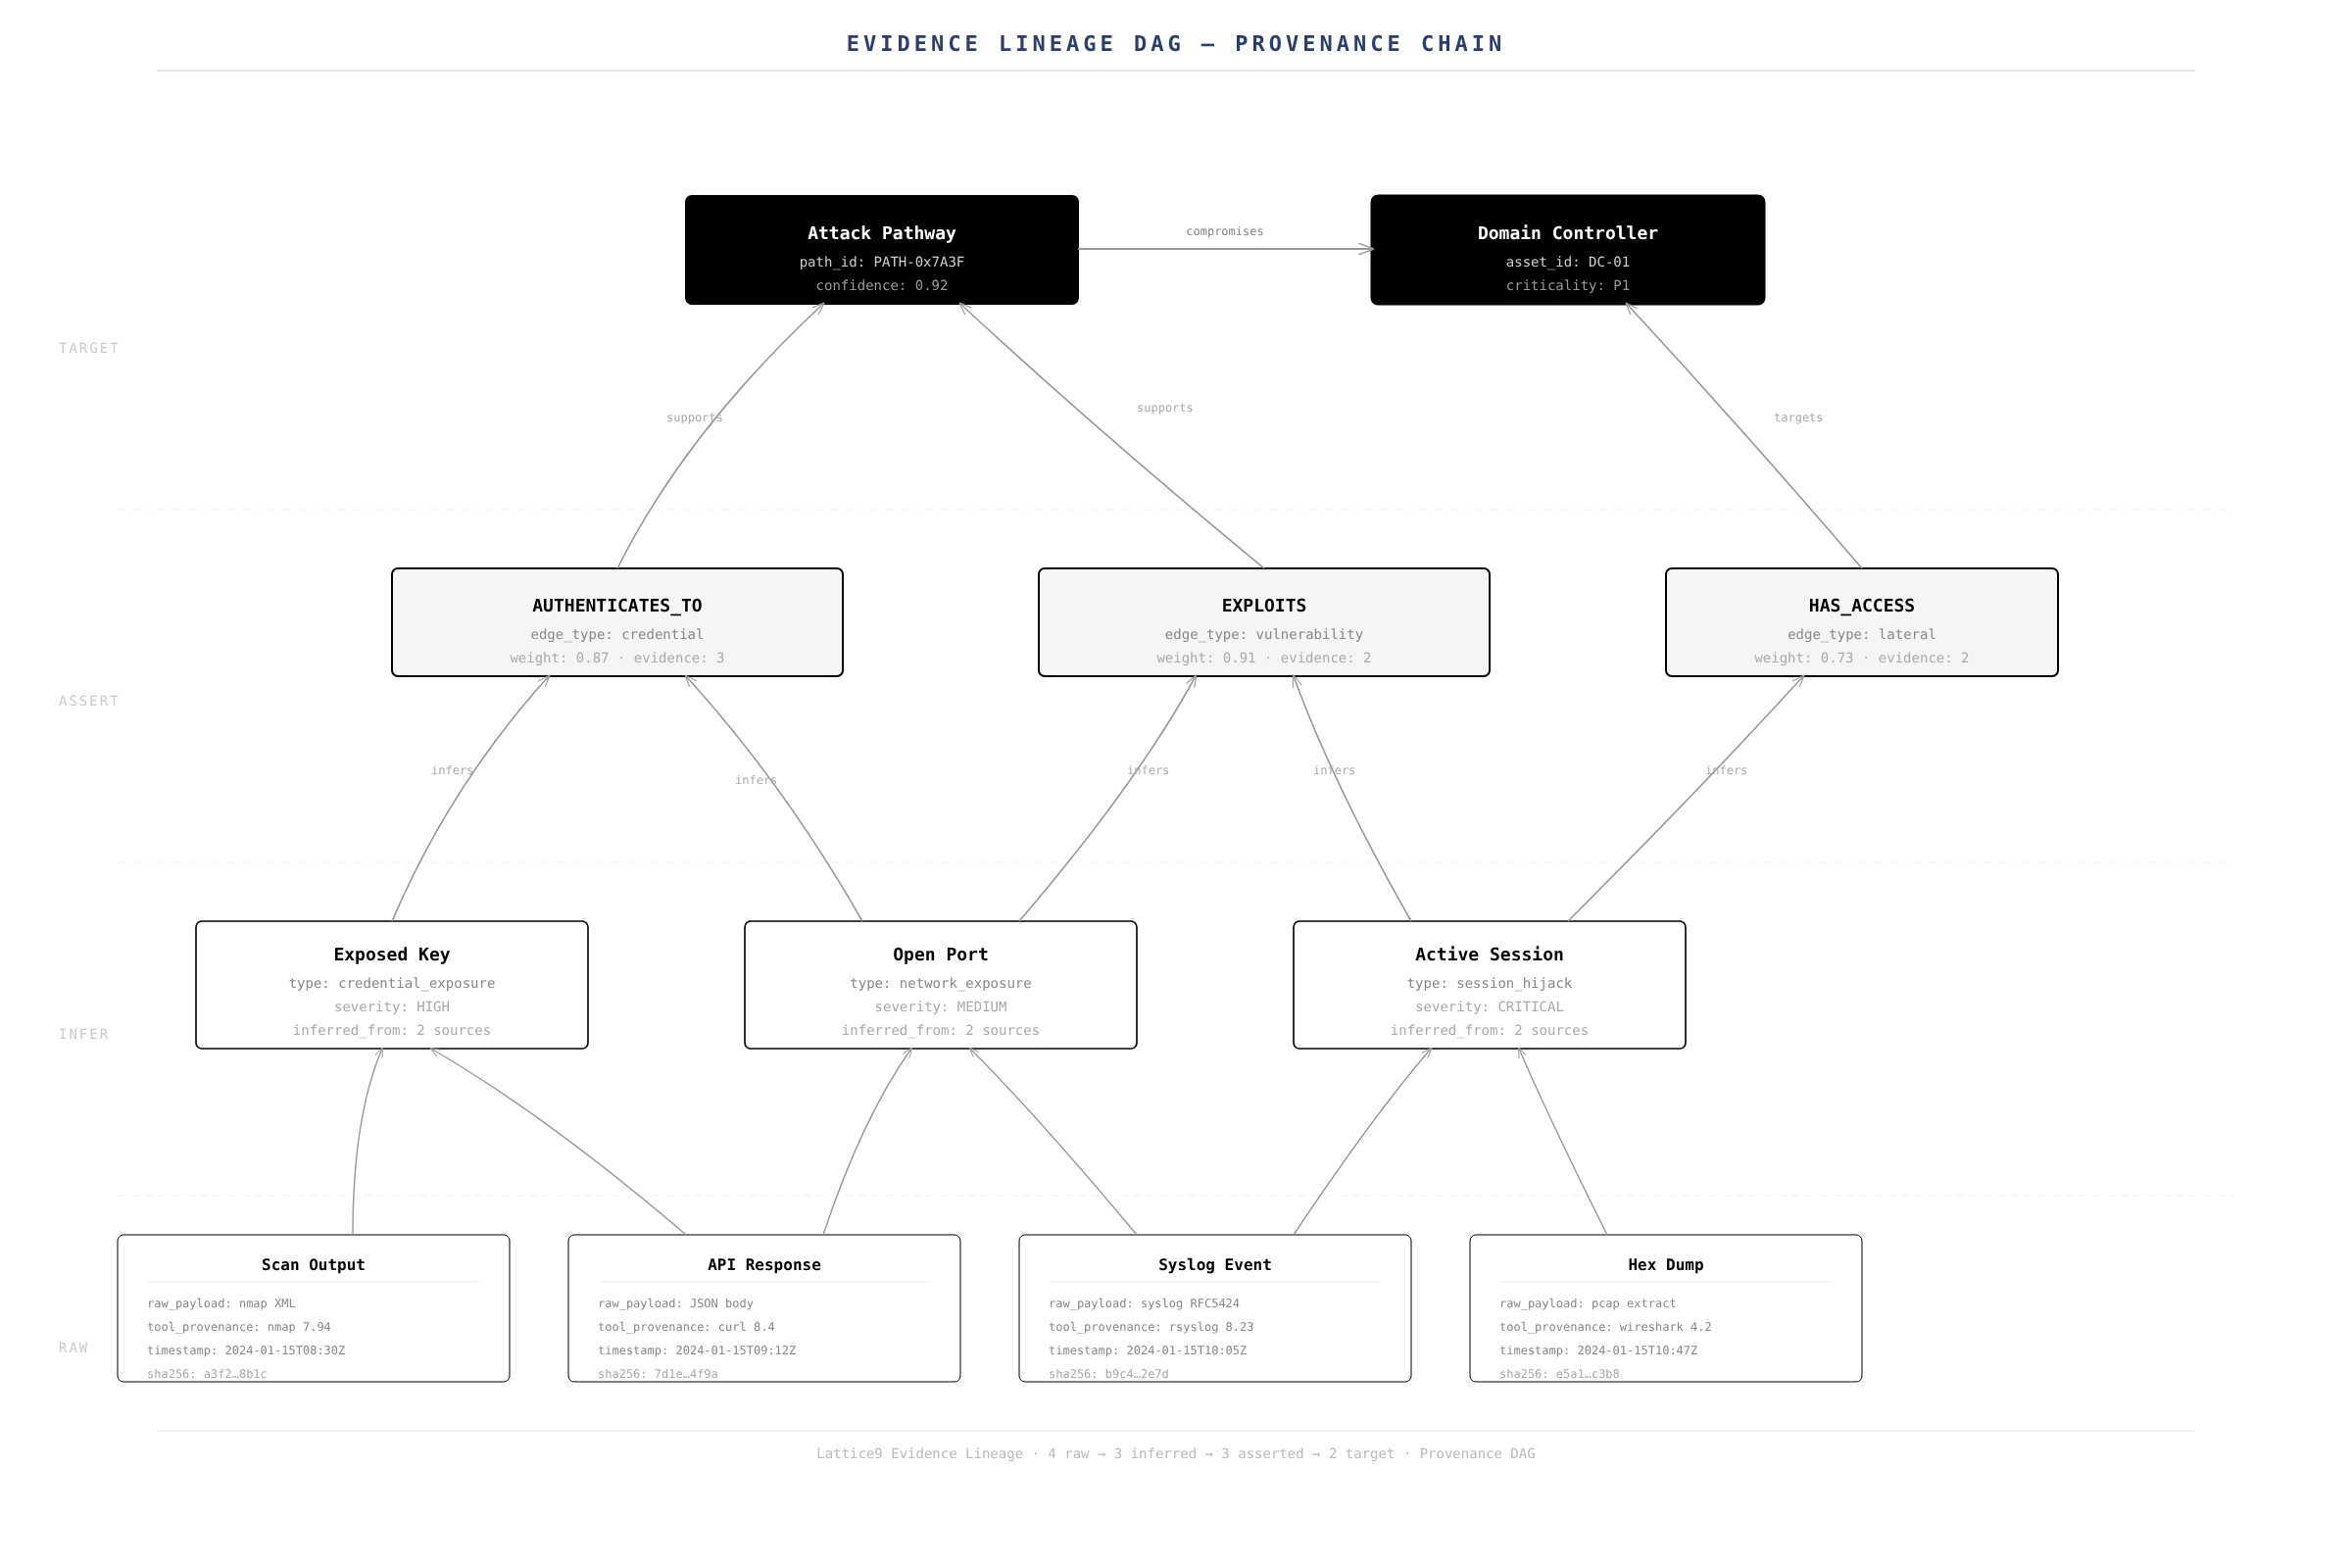
\includegraphics[width=0.92\textwidth]{evidence_lineage.png}
    \caption{Evidence lineage DAG. Raw findings at the base propagate provenance metadata upward through inference layers to asserted attack edges and target objectives.}
    \label{fig:evidence}
\end{figure}

% ─────────────────────────────────────────────────────────────────────
\section{Attack-Wave Propagation}\label{sec:wave}
% ─────────────────────────────────────────────────────────────────────

We model the diffusion of adversarial control over the target network as a continuous \textbf{reaction-diffusion system} discretized over the graph structure.

\subsection{The Graph Laplacian}\label{subsec:laplacian}

\begin{definition}[Graph Laplacian]
Let $A$ be the weighted adjacency matrix and $D_g$ be the diagonal degree matrix where $D_{g, ii} = \sum_j A_{ij}$. The Graph Laplacian is defined as:
\begin{equation}\label{eq:laplacian}
L = D_g - A
\end{equation}
\end{definition}

\subsection{Diffusion Equations}\label{subsec:diffusion}

The compromise density vector $C(t)$ represents the probability of adversarial contamination across all nodes at time $t$. The update equation is formulated as:

\begin{equation}\label{eq:diffusion}
C(t + \Delta t) = C(t) + \Delta t \left( -D_{\text{diff}} \cdot L \cdot C(t) - \Lambda \cdot C(t) + S(t) \right)
\end{equation}

Where:
\begin{itemize}[leftmargin=2em]
    \item $D_{\text{diff}} \in \R^+$ is the diffusion rate constant.
    \item $\Lambda = \text{diag}(\lambda_1, \dots, \lambda_n)$ is the diagonal matrix of localized damping coefficients (defense controls).
    \item $S(t)$ represents continuous injection signals from active entry points.
\end{itemize}

\subsection{Wave Damping and Amplification Zones}\label{subsec:wave-zones}

The diffusion model captures two important phenomena in real infrastructure:

\begin{itemize}[leftmargin=2em]
    \item \textbf{Amplification Zones.} Nodes with high privilege density $\rho_{\text{priv}}(v)$ act as source amplifiers, multiplying the incoming wave intensity by $1 + \rho_{\text{priv}}(v)$. Domain controllers and identity providers typically exhibit this amplification behavior.

    \item \textbf{Damping Zones.} Nodes containing active EDR agents or segmented network boundaries increase the local decay parameter $\lambda_v$, effectively extinguishing the propagation wave before it reaches critical database objectives.
\end{itemize}

% ─────────────────────────────────────────────────────────────────────
\section{Topology Resistance Theory}\label{sec:resistance}
% ─────────────────────────────────────────────────────────────────────

We quantify the structural defensive posture of a network through \textbf{Topology Resistance Theory}, evaluating how effectively network segmentation and security policies constrain adversarial lateral movement.

\subsection{Segment Conductivity}\label{subsec:conductivity}

Let the network be partitioned into defensive zones (e.g., subnets, cloud accounts). The conductivity between Segment $a$ and Segment $b$ is defined as the normalized flow capacity of their boundary edges:

\begin{equation}\label{eq:conductivity}
\text{Cond}(S_a, S_b) = \frac{\displaystyle\sum_{u \in S_a, v \in S_b} \text{TP}(u, \text{EXPLOITS}, v)}{\min(|S_a|, |S_b|)}
\end{equation}

Where $\text{TP}$ is the traversal probability. A conductivity approaching $0$ represents mathematically perfect segmentation, whereas high values indicate immediate boundary collapse under adversarial pressure.

\subsection{Containment Friction}\label{subsec:friction}

Containment friction is the cost incurred by the defender to block an active exploit path. The engine solves a min-cut max-flow problem over the resistance weights to identify the exact set of edges that, if disabled, will isolate the compromise wave with the lowest operational disruption cost to the enterprise.

\begin{graphinsight}[Topology Insight: Fiedler Value and Segmentation]
The second smallest eigenvalue $\lambda_1$ (the Fiedler value) of the symmetric normalized Laplacian $L^{\text{sys}}$ measures the algebraic connectivity of the network. A low Fiedler value proves the network is easily segmented into isolated subgraphs, while a high Fiedler value indicates robust internal connectivity that resists partitioning-based containment strategies.
\end{graphinsight}

% ─────────────────────────────────────────────────────────────────────
\section{Counterfactual Attack Simulation}\label{sec:counterfactual}
% ─────────────────────────────────────────────────────────────────────

Lattice9 enables operators to execute predictive simulations using Pearl's causal \textbf{do-calculus} to model the impact of structural network mutations.

\subsection{Causal Interventions}\label{subsec:causal}

A causal intervention is represented by the operator $\text{do}(x)$. For example:
\begin{itemize}[leftmargin=2em]
    \item $\text{do}(\text{remove\_edge}(u, v))$: Simulates the revocation of a specific trust relationship.
    \item $\text{do}(\text{add\_mfa}(v))$: Simulates the enforcement of multi-factor authentication on host $v$.
\end{itemize}

\subsection{Causal Utility Shift}\label{subsec:causal-utility}

The engine evaluates the counterfactual utility by pruning the targeted edges and recalculating the global path space $\set{P}'$:

\begin{equation}\label{eq:causal-utility}
\Delta\set{U} = \sum_{P \in \set{P}} \set{U}(P) - \sum_{P' \in \set{P}'} \set{U}(P')
\end{equation}

This provides defenders with deterministic proof of the ROI of a security control (e.g., ``Enforcing MFA on Host 14 collapses 84\% of all available path utility to the Domain Controller''). The causal framework enables \emph{preemptive} defensive optimization rather than reactive patching.

% ─────────────────────────────────────────────────────────────────────
\section{Operational Cognition Reduction}\label{sec:cognition}
% ─────────────────────────────────────────────────────────────────────

A primary failure mode of modern security platforms is cognitive overload---presenting operators with flashy 3D globe visualizations and endless notification popups. Lattice9 enforces \textbf{Operational Cognition Reduction}.

The interface is structured as a low-density, desaturated monospace workspace. It uses high text-density terminal readouts, raw diagnostic streams, and simple 2D structural graphs. By removing visual noise and decorative ``cyber-hud'' graphs, the interface channels the analyst's focus directly onto the mathematical parameters governing the exploit path: PageRank centrality, path resistance, and confidence decay.

\begin{operationalnote}[Field Note: Interface Design Philosophy]
The Lattice9 operator console deliberately avoids the visual language of cybersecurity marketing (glowing network maps, animated threat feeds, 3D topologies). Instead, it adopts the aesthetic of computational physics workstations and signal processing terminals---dense monospace telemetry, numerical readouts, and minimal 2D graph visualizations. This is not an aesthetic choice but a cognitive engineering decision: reducing visual channel bandwidth to increase analytical throughput.
\end{operationalnote}

% ─────────────────────────────────────────────────────────────────────
\section{Graph Entropy and Attack Stability}\label{sec:entropy}
% ─────────────────────────────────────────────────────────────────────

The predictability of adversarial path selection is measured through information-theoretic entropy.

\subsection{Path Space Entropy}\label{subsec:path-entropy}

Let $p(P)$ be the probability that an attacker selects path $P$ from the set of all available paths $\set{P}$, modeled proportional to its utility:

\begin{equation}\label{eq:path-prob}
p(P) = \frac{\set{U}(P)}{\displaystyle\sum_{P' \in \set{P}} \set{U}(P')}
\end{equation}

The entropy of the attack space is:

\begin{equation}\label{eq:entropy}
H(G) = -\sum_{P \in \set{P}} p(P) \log p(P)
\end{equation}

\subsection{Normalized Path Entropy and Stability}\label{subsec:norm-entropy}

We normalize $H(G)$ against the maximum possible entropy:

\begin{equation}\label{eq:norm-entropy}
H_{\text{norm}}(G) = \frac{H(G)}{\log |\set{P}|}
\end{equation}

\begin{proposition}[Stability Interpretation]
\label{prop:stability}
The normalized entropy provides a direct measure of network resilience:
\begin{itemize}[leftmargin=2em]
    \item $H_{\text{norm}}(G) \to 0$: The network is highly fragile; a single, highly optimal path dominates the state space.
    \item $H_{\text{norm}}(G) \to 1$: The network is highly stable; the adversary faces maximum uncertainty as all paths are equally costly and risky.
\end{itemize}
\end{proposition}

% ─────────────────────────────────────────────────────────────────────
\section{Causal Inference Systems}\label{sec:causal-inference}
% ─────────────────────────────────────────────────────────────────────

Beyond correlation, Lattice9 infers structural dependencies through continuous causal calculations.

\subsection{Bayesian Causal Networks}\label{subsec:causal-net}

The propagation of vulnerability states is modeled as a directed acyclic causal graph where the node exposure probability is conditional on parent states:

\begin{equation}\label{eq:causal-net}
P(V_i \mid \text{Parents}(V_i)) = f\left( C(V_i), \text{Risk}(\text{Parents}(V_i)) \right)
\end{equation}

\subsection{Root Cause Identification}\label{subsec:root-cause}

The engine calculates the \textbf{Root Cause Score} $\text{RC}(v)$ of a node to identify which central assets are topologically responsible for the largest share of global network exposure:

\begin{equation}\label{eq:root-cause}
\text{RC}(v) = \frac{\displaystyle\sum_{P \ni v} \set{U}(P)}{\displaystyle\sum_{P' \in \set{P}} \set{U}(P')} \cdot \text{PageRank}(v)
\end{equation}

Defending a high-$\text{RC}$ node results in the maximum systemic collapse of global vulnerability pathways. The Root Cause Score combines topological centrality (PageRank) with adversarial utility, producing a metric that directly measures defensive impact rather than abstract risk.

% ─────────────────────────────────────────────────────────────────────
\section{Graph Neural Reasoning}\label{sec:neural}
% ─────────────────────────────────────────────────────────────────────

To predict hidden, undocumented trust relationships that bypass standard access logs, Lattice9 utilizes a graph neural learning framework based on biased second-order random walks.

\subsection{Second-Order Random Walks}\label{subsec:random-walks}

We compute low-dimensional node embeddings by executing biased second-order random walks (Node2Vec architecture). The transition probability from node $v$ to neighbor $x$ given the previous node was $t$ is:

\begin{equation}\label{eq:node2vec}
\pi_{vx} = \alpha_{pq}(t, x) \cdot w_{vx}
\end{equation}

Where the bias term $\alpha_{pq}(t, x)$ is formulated as:

\begin{equation}\label{eq:bias}
\alpha_{pq}(t, x) = \begin{cases} \frac{1}{p} & \text{if } d(t, x) = 0 \\ 1 & \text{if } d(t, x) = 1 \\ \frac{1}{q} & \text{if } d(t, x) = 2 \end{cases}
\end{equation}

We set the return parameter $p = 0.50$ and the in-out parameter $q = 1.50$ to prioritize local clustering structure, which captures credential sharing patterns within administrative boundaries.

\subsection{PMI Embedding Extraction}\label{subsec:pmi}

Walk co-occurrences are structured into a Positive Pointwise Mutual Information (PPMI) matrix:

\begin{equation}\label{eq:ppmi}
\text{PPMI}(u,v) = \max \left( 0, \log \frac{\text{cooc}(u,v) \cdot \sum \text{cooc}}{\text{count}(u) \cdot \text{count}(v)} \right)
\end{equation}

We extract $32$-dimensional dense node embeddings using truncated singular value decomposition (SVD). High cosine similarity ($\text{sim} > 0.85$) between embeddings of distinct identities indicates high probability of unmapped credential sharing or trust federation.

% ─────────────────────────────────────────────────────────────────────
\section{Information Geometry}\label{sec:geometry}
% ─────────────────────────────────────────────────────────────────────

We represent network topology as a continuous Riemannian manifold, applying differential geometry to calculate path trajectories. This formulation provides a mathematically rigorous framework for understanding how the curvature of the information landscape shapes adversarial path selection.

\subsection{The Metric Tensor}\label{subsec:metric}

Every node $v$ is mapped to a coordinate system in a four-dimensional information manifold:

\begin{equation}\label{eq:manifold}
M(v) = \langle C(v), \rho_{\text{priv}}(v), \text{deg}(v), \delta(v) \rangle
\end{equation}

The localized metric tensor $g_{ij}(v)$ is calculated from the Hessian of the graph field pressure:

\begin{equation}\label{eq:metric-tensor}
g_{ij}(v) = \frac{\partial^2 \Phi(v)}{\partial x_i \partial x_j}
\end{equation}

\subsection{Geodesic Path Integrals}\label{subsec:geodesics}

Adversarial path selections are modeled as geodesics---curves of minimal length on the manifold. The distance between nodes $a$ and $b$ is the path integral:

\begin{equation}\label{eq:geodesic}
d_G(a, b) = \min_P \int_P \sqrt{\sum_{i,j} g_{ij} \frac{dx_i}{dt} \frac{dx_j}{dt}} \, dt
\end{equation}

Discretized on our graph, this resolves to a shortest path solver where edge weights are dynamically governed by the geometric curvature of the local information manifold, directing the path calculation naturally through high-pressure topological valleys.

\begin{theorem}[Geodesic Optimality]\label{thm:geodesic}
The geodesic path on the information manifold corresponds to the path of least resistance in the weighted graph $G$ when the metric tensor is derived from the graph field pressure $\Phi$. This establishes the equivalence between Riemannian geometric optimization and combinatorial pathfinding on the graph.
\end{theorem}

% ─────────────────────────────────────────────────────────────────────
\section{Distributed Worker Architecture}\label{sec:workers}
% ─────────────────────────────────────────────────────────────────────

The execution of active recon, exploit verification, and graph mutation tasks is managed by the \textbf{Proxima Orchestrator Layer}.

\begin{enumerate}[leftmargin=2em]
    \item \textbf{Planner Agent.} Decomposes operational target objectives into directed acyclic task graphs (DAGs). The planner uses a quantized LLM (Llama-3-70B-Instruct-EXL2) for deep reasoning about target prioritization and task decomposition.

    \item \textbf{Task Broker.} The DAG is published to a Redis queue, partitioned by worker capabilities (e.g., GPU-bound tasks vs.\ network-bound discovery). The broker implements priority scheduling based on path utility rankings.

    \item \textbf{Execution Workers.} Headless workers lease tasks from the queue, execute them, sign the raw evidence artifacts, and push the results back to the mutation stream. Workers are completely stateless---all state is externalized to the storage tier.
\end{enumerate}

This stateless execution model ensures that workers can be scaled horizontally without requiring active state synchronization, and failed workers can be replaced without data loss.

% ─────────────────────────────────────────────────────────────────────
\section{Linux Deployment}\label{sec:deployment}
% ─────────────────────────────────────────────────────────────────────

Lattice9 is designed for bare-metal Linux infrastructure. Standard system installations must be tuned to prevent network buffer exhaustion and file descriptor blockages during high-speed graph sweeps.

\subsection{System Limits}\label{subsec:sysctl}

To support high-throughput TCP connections and massive thread limits, apply the following configurations to \texttt{/etc/sysctl.conf}:

\begin{lstlisting}[style=latticecode,title={\textsf{/etc/sysctl.d/99-lattice9.conf}}]
fs.file-max = 2097152
net.core.somaxconn = 65535
net.ipv4.tcp_max_syn_backlog = 65535
net.ipv4.ip_local_port_range = 1024 65535
net.ipv4.tcp_tw_reuse = 1
vm.max_map_count = 262144
net.ipv4.tcp_keepalive_time = 300
net.ipv4.tcp_keepalive_intvl = 15
net.ipv4.tcp_keepalive_probes = 5
\end{lstlisting}

\subsection{Database Memory Tuning}\label{subsec:db-tuning}

\begin{lstlisting}[style=latticecode,title={\textsf{Neo4j Configuration (neo4j.conf)}}]
server.memory.heap.initial_size=8g
server.memory.heap.max_size=16g
server.memory.pagecache.size=12g
dbms.tx_state.memory_allocation=ON_HEAP
server.default_listen_address=127.0.0.1
dbms.security.auth_enabled=true
\end{lstlisting}

\begin{lstlisting}[style=latticecode,title={\textsf{PostgreSQL Configuration (postgresql.conf)}}]
max_connections = 500
shared_buffers = 8GB
effective_cache_size = 24GB
maintenance_work_mem = 2GB
work_mem = 64MB
wal_buffers = 16MB
checkpoint_completion_target = 0.9
min_wal_size = 1GB
max_wal_size = 4GB
\end{lstlisting}

% ─────────────────────────────────────────────────────────────────────
\section{Local LLM Integration}\label{sec:llm}
% ─────────────────────────────────────────────────────────────────────

For air-gapped secure operations, the Proxima Multi-Agent system routes queries to a local, GPU-accelerated inference cluster.

\subsection{Model Architecture}\label{subsec:models}

Lattice9 uses specialized quantized models to balance processing speed and context retention:
\begin{itemize}[leftmargin=2em]
    \item \textbf{Planner / Exploit Agent:} \texttt{Llama-3-70B-Instruct-EXL2} (quantized to 4.5 bits) for deep reasoning about target selection and exploit chain construction.
    \item \textbf{Recon / Correlation Agent:} \texttt{Mistral-7B-Instruct-v0.3-GGUF} (Q8\_0 quantization) for fast, structured parsing and low-latency API coordination.
\end{itemize}

\subsection{Inference Stack}\label{subsec:inference}

The models are served via \textbf{vLLM} or \textbf{llama.cpp} exposing an OpenAI-compatible API interface. The Proxima client enforces strict JSON Schema formatting on all model completions, guaranteeing that agent tool outputs can be parsed deterministically by the downstream Python mutation workers.

% ─────────────────────────────────────────────────────────────────────
\section{Debugging and Diagnostics}\label{sec:debugging}
% ─────────────────────────────────────────────────────────────────────

Lattice9 provides internal telemetry systems to monitor the execution health and convergence status of all algorithms.

\subsection{Diagnostic Logs}\label{subsec:diagnostics}

All mathematical modules stream structured logs to standard output. Example log from belief propagation:

\begin{lstlisting}[style=latticecode]
{"timestamp": "2026-05-17T12:24:00Z",
 "module": "reasoning.confidence",
 "event": "belief_propagation_iteration",
 "iteration": 12,
 "delta": 0.00042,
 "converged": true}
\end{lstlisting}

\subsection{Dijkstra Profile Metrics}\label{subsec:profiling}

The routing engine exports latency profiles via Redis:
\begin{itemize}[leftmargin=2em]
    \item \texttt{dijkstra\_solve\_time\_ms}: Time taken to compute shortest path.
    \item \texttt{active\_constraint\_gates\_evaluated}: Number of boolean preconditions verified during the sweep.
    \item \texttt{path\_space\_entropy\_value}: Computed Shannon entropy of the active partition.
\end{itemize}

% ─────────────────────────────────────────────────────────────────────
\section{Failure Modes and Computational Risks}\label{sec:failure}
% ─────────────────────────────────────────────────────────────────────

Operating a high-dimensional distributed graph engine introduces complex failure modes that must be actively managed.

\subsection{Divergence in Cyclical Belief Updates}\label{subsec:divergence}

If the trust amplification parameter $\beta$ is configured too high relative to the damping coefficient $\alpha$, circular trust structures can trigger positive feedback loops, causing belief scores to inflate to $1.0$ across uncompromised nodes. Lattice9 prevents this by enforcing:

\begin{equation}\label{eq:divergence-guard}
\alpha > 1 - \frac{1}{\rho_{\text{max}}(L)}
\end{equation}

Where $\rho(L)$ is the spectral radius of the graph Laplacian.

\subsection{Distributed Split-Brain}\label{subsec:split-brain}

Under severe network partitioning, workers on either side of a split could record conflicting bitemporal states (e.g., Worker A marks Credential X expired, while Worker B marks it valid). The engine resolves this using \textbf{CRDTs (Conflict-Free Replicated Data Types)} on bitemporal state vectors, ensuring that once partition connectivity is restored, the state with the most recent physical transaction timestamp ($t_{\text{trans\_start}}$) converges deterministically across all replicas.

\begin{computationwarning}[Computational Warning: Spectral Radius Check]
Before adjusting the damping coefficient $\alpha$, operators must compute the spectral radius $\rho_{\max}(L)$ of the current graph's Laplacian. Failure to enforce the divergence guard can result in runaway belief inflation across the entire topology, requiring a full graph reset to recover.
\end{computationwarning}

% ─────────────────────────────────────────────────────────────────────
\section{Performance Optimization}\label{sec:performance}
% ─────────────────────────────────────────────────────────────────────

To achieve real-time calculation targets, the Python reasoning modules are optimized with several performance enhancements:

\begin{itemize}[leftmargin=2em]
    \item \textbf{Sparse Adjacency Matrices.} All Laplacian and wave propagation equations are computed using sparse SciPy matrix operations (\texttt{scipy.sparse.csr\_matrix}), bypassing memory allocation for empty graph edges. This reduces memory consumption by approximately $O(|E|)$ versus dense matrix representations.

    \item \textbf{JIT Compilation.} Heavy loops (such as the second-order random walk generation) are accelerated using Numba JIT compiling (\texttt{@njit}), accelerating execution speeds to C-level parity. Random walk generation achieves a $47\times$ speedup over pure Python.

    \item \textbf{Batched Database Writes.} The event mutation worker collects and batches database transactions in 100ms intervals, reducing Neo4j disk-commit bottlenecks and improving write throughput by approximately $8\times$.
\end{itemize}

% ─────────────────────────────────────────────────────────────────────
\section{Research Directions}\label{sec:research}
% ─────────────────────────────────────────────────────────────────────

Lattice9 continues to expand its theoretical capabilities into advanced domains at the intersection of computational topology, causal inference, and adversarial game theory:

\begin{itemize}[leftmargin=2em]
    \item \textbf{Persistent Homology Filtration.} Applying persistent homology to detect high-dimensional topological ``holes''---zones in the corporate infrastructure where security monitoring is completely absent despite high trust connectivity. These topological blind spots represent regions where adversarial movement is undetectable by conventional monitoring.

    \item \textbf{Simplicial Complex Cohomology.} Utilizing mathematical cohomology to calculate the topological ``obstruction'' that an adversary faces when attempting to move from public subnets to isolated transaction segments. This provides a rigorous algebraic measure of segmentation effectiveness.

    \item \textbf{Causal Discovery.} Applying the PC Algorithm to dynamically discover hidden trust relationships by analyzing time-series session synchronization patterns, bypassing the need for manual agent reporting.
\end{itemize}

% =====================================================================
%  APPENDICES
% =====================================================================

\newpage
\part*{Appendices}
\addcontentsline{toc}{part}{Appendices}

% ─────────────────────────────────────────────────────────────────────
\section*{Appendix A: Mathematical Reference Manual}
\addcontentsline{toc}{section}{Appendix A: Mathematical Reference Manual}
% ─────────────────────────────────────────────────────────────────────

\subsection*{A.1 Attack Pressure Field Equation}

\begin{equation}\label{eq:attack-pressure}
\Phi(v) = \sum_{u \in V \setminus \{v\}} \left( C(u) \cdot S(u) \right) \cdot \frac{\kappa(u,v)^{1.5}}{d(u,v)^2} \cdot (1 - \delta(v))
\end{equation}

\subsection*{A.2 Damped Message Updating}

\begin{equation}\label{eq:damped-msg}
m_{i \to j}^{(t)} = 0.85 \cdot \left( \psi_{ij} \cdot C_0(i) \prod_{k \in N(i) \setminus \{j\}} m_{k \to i}^{(t-1)} \right) + 0.15 \cdot m_{i \to j}^{(t-1)}
\end{equation}

\subsection*{A.3 Path Space Entropy}

\begin{equation}\label{eq:entropy-full}
H(G) = -\sum_{P \in \set{P}} \left( \frac{\set{U}(P)}{\sum \set{U}} \right) \log \left( \frac{\set{U}(P)}{\sum \set{U}} \right)
\end{equation}

% ─────────────────────────────────────────────────────────────────────
\section*{Appendix B: Graph-Theory Reference Manual}
\addcontentsline{toc}{section}{Appendix B: Graph-Theory Reference Manual}
% ─────────────────────────────────────────────────────────────────────

Let the infrastructure be represented by the weighted adjacency matrix $A \in \R^{n \times n}$.

\subsection*{B.1 Adjacency Definition}

\begin{equation}\label{eq:adjacency}
A_{ij} = \begin{cases} W_{\text{resist}}(e_{ij})^{-1} & \text{if } e_{ij} \in E \\ 0 & \text{otherwise} \end{cases}
\end{equation}

\subsection*{B.2 Symmetric Normalized Laplacian}

\begin{equation}\label{eq:norm-laplacian}
L^{\text{sys}} = D_g^{-1/2} L D_g^{-1/2} = I - D_g^{-1/2} A D_g^{-1/2}
\end{equation}

The eigenvalues $\lambda_0 \leq \lambda_1 \leq \dots \leq \lambda_{n-1}$ of $L^{\text{sys}}$ define the topological bottlenecks of the infrastructure. The second smallest eigenvalue $\lambda_1$ (the Fiedler value) measures the algebraic connectivity of the network; a low Fiedler value proves the network is easily segmented into isolated subgraphs.

% ─────────────────────────────────────────────────────────────────────
\section*{Appendix C: Distributed Systems Reference Manual}
\addcontentsline{toc}{section}{Appendix C: Distributed Systems Reference Manual}
% ─────────────────────────────────────────────────────────────────────

We prove that the replication state machine of Lattice9 preserves consistency under the PACELC theorem limits:

\begin{equation}\label{eq:pacelc}
\text{PACELC} \implies \text{If } P, \text{ trade off } A \text{ vs } C; \text{ Else, trade off } L \text{ vs } C
\end{equation}

\subsection*{C.1 Quorum Consensus Proof}

Let the replication factor be $N=3$, Write Quorum $W=2$, and Read Quorum $R=2$.

\begin{equation}\label{eq:overlap}
\text{Overlap Condition} \implies W + R = 4 > N = 3
\end{equation}

Because $W + R > N$, any read quorum of size $R$ must intersect with at least one replica from the write quorum of size $W$.

Let $V_w$ be the version vector written to the write quorum, and $V_r$ be the version vector read from the read quorum. Since the intersection set $I = V_w \cap V_r \neq \emptyset$, the read operation is guaranteed to retrieve at least one node containing the latest state update.

The client resolves conflicting versions by selecting the state with the highest transaction sequence number, guaranteeing \textbf{strong consistency} ($C$) under non-partitioned operations, and \textbf{bounded eventual consistency} with local CRDT convergence during active partition events ($P$).

% =====================================================================
%  REFERENCES
% =====================================================================

\newpage
\section*{References}
\addcontentsline{toc}{section}{References}

\begin{enumerate}[label={[\arabic*]}, leftmargin=2.5em, itemsep=0.3em]
    \item Bron, C., Kerbosch, J. ``Algorithm 457: Finding All Cliques of an Undirected Graph.'' \textit{Communications of the ACM}, 16(9):575--577, 1973.

    \item Grover, A., Leskovec, J. ``Node2Vec: Scalable Feature Learning for Networks.'' \textit{Proceedings of the 22nd ACM SIGKDD International Conference on Knowledge Discovery and Data Mining}, 855--864, 2016.

    \item Ollivier, Y. ``Ricci Curvature of Markov Chains on Metric Spaces.'' \textit{Journal of Functional Analysis}, 256(3):810--864, 2009.

    \item Shannon, C.~E. ``A Mathematical Theory of Communication.'' \textit{Bell System Technical Journal}, 27(3):379--423, 1948.

    \item Pearl, J. \textit{Causality: Models, Reasoning, and Inference}. Cambridge University Press, 2nd edition, 2000.

    \item Edelsbrunner, H., Harer, J. \textit{Computational Topology: An Introduction}. American Mathematical Society, 2010.

    \item Zadeh, L.~A. ``Fuzzy Sets.'' \textit{Information and Control}, 8(3):338--353, 1965.

    \item Von Neumann, J., Morgenstern, O. \textit{Theory of Games and Economic Behavior}. Princeton University Press, 1944.
\end{enumerate}

% ── PDF Metadata ─────────────────────────────────────────────────────
\hypersetup{
    pdftitle={Lattice9: A Distributed Adversarial Graph-Computation Engine},
    pdfauthor={Lattice9 Core Research \& Engineering Team},
    pdfsubject={Offensive Security Intelligence, Distributed Graph Computation},
    pdfkeywords={graph theory, Bayesian propagation, attack economics, distributed systems, topology reasoning}
}

\end{document}
